\chapter{Local Inference of Language Models}
\label{sec:local}

% Source notes: Vault/wiki concepts On-Device Inference, Local Inference Hardware, Prefill and Decode, Open-Weight Models,
% Small Language Models, Quantization, Privacy and Data Sovereignty, Navier-Stokes Credit Dispute (2026), Energy of LLM
% Inference; figures from `groundone figures locality` (Project/GroundOne/src/groundone/figures/locality.py).
% Hardware specifications: vendor pages accessed 2026-10-11 (Vault/raw/local_inference).

This thesis builds a verifier that runs entirely on the user's own machine, and this choice shapes every other one: the
size of the models, the way decisions are read from them, the measurements and the comparisons. This chapter explains
why local inference matters, what makes it possible today and what it costs. It starts from the reasons for keeping a
model on the device and from the open-weight models that make this possible. It then derives a simple cost model of
inference on one device, which shows why reading a token costs far less than writing one, and surveys the hardware on which
local models run, from the laptop used in this work to dedicated desktop machines. It continues with the software and
the quantisation that bring models within reach of that hardware, and with energy. It closes by drawing the consequence
for verification, which motivates the design of GroundOne in the following chapters.

\section{From hosted to local models}
\label{sec:local-why}

Most people use language models through hosted services. The user's input travels over the network to a provider, a
model in a datacenter processes it, and the answer travels back. The model, the hardware and the policies that govern
the data all belong to the provider. Running the model on the user's own device changes all of this at once. Five
properties follow, and each of them matters for a retrieval-augmented assistant that works on private documents.

\paragraph{Privacy as a technical guarantee.} With a hosted model, every document and every question is sent to a
third party, and what happens to them afterwards, how long they are kept, who can access them and whether they are used
to improve future models, is governed by contract and policy. The user can read the policy but cannot verify that it is
respected. With a local model the documents never leave the machine, so the question does not arise: privacy becomes a
property of the system rather than a promise. Surveys of edge intelligence, that is, of running models on peripheral
devices close to the user, state the point directly: on-device inference eliminates privacy leakage and the need for an
Internet connection~\cite{qu2025mobileedge}.

European law makes the difference concrete. Under the General Data Protection Regulation (GDPR), the processing of
personal data explicitly includes its ``disclosure by transmission''~\cite[Art.~4(2)]{gdpr2016}. Sending a document that
contains personal data to a hosted model therefore makes the provider a processor\footnote{In the GDPR, the
\emph{controller} decides why and how personal data are processed; the \emph{processor} processes them on behalf of the
controller, for instance by providing a computing service.}, bound by a contract with the specific guarantees of
Article~28. If, in addition, the provider operates outside the European Union, the transfer of the data must have a legal
basis: an adequacy decision\footnote{A decision by which the European Commission recognises that a third country ensures
a level of data protection essentially equivalent to that of the European Union.}, appropriate safeguards or one of the
derogations provided by Articles~44--49~\cite{gdpr2016}. A verifier that runs on the user's device involves no processor
and no transfer. It does not remove every obligation, since the
organisation that uses it must still respect the principles of Article~5 and secure the device, but it removes the
obligations that depend on trusting someone else. Many confidential documents, such as unpublished research, contracts
or source code, contain no personal data at all; for them the regulation does not apply, and the argument becomes one
of confidentiality.

A recent episode illustrates what is at stake. In September 2026 OpenAI announced that an internal multi-agent system had
produced a proof of blow-up (the formation of a singularity in finite time) for the forced Navier--Stokes equations, one of the Millennium Prize problems, formalised in
the Lean proof assistant~\cite{rits2026navierstokes}. Two mathematicians, Tristan Buckmaster and Levent Alpöge, had
released related results for the Euler equations at about the same time, and disputed the credit. Buckmaster had written his
drafts in OpenAI's own coding assistant, and asked the company ``whether the model had been trained on, or had access
to, our sessions in Codex, into which we had been putting all our drafts''~\cite{kahn2026navierstokes}. OpenAI denied
that its researchers or agents had seen the work before its release, but added: ``While unlikely, we cannot rule out
that de-identified data derived from their usage of our products helped improve our
models''~\cite{rits2026navierstokes,capella2026navierstokes}. Nothing in the public record shows that the drafts were
misused, and the dispute is mainly about credit. What the episode does show is that, once unpublished work is inside a
hosted model, neither the user nor, by its own statement, the provider can exclude that it contributed to the provider's
models. With a local model this question cannot be asked.

Providers are aware of the problem. Apple describes on-device processing as the cornerstone of its approach to privacy,
and for requests that exceed the device it built Private Cloud Compute, a dedicated cloud with custom servers, no
privileged access for staff, no persistent storage of requests and a public log of the software images that run on
it~\cite{apple2024pcc}. The design is a serious attempt to make hosted inference verifiable, and its very complexity is
an argument for locality. Privacy in the cloud requires custom silicon, a hardened operating system and cryptographic
attestation, that is, a signed proof of which software is running on the servers. Even so, the system rests on trust in
the hardware, in the supply chain and in the attestation itself, which only security researchers, not users, can
inspect~\cite{apple2024pcc}.

\paragraph{Availability.} A local model works without a network and without depending on the availability of a
provider. For an assistant used on a train, in a hospital ward with restricted connectivity or in an air-gapped
environment, that is, one physically isolated from any network, this is a requirement rather than a convenience.

\paragraph{Stability and reproducibility.} The weights of a local model change only when the user changes them. A
hosted model can be updated, re-tuned or withdrawn at any time, often silently, so that the same request produces a
different answer from one month to the next. For a verifier whose thresholds are calibrated on development data
(Chapter~\ref{sec:method}), a silent change of the underlying model would invalidate the calibration without warning.

\paragraph{Cost.} A hosted model is paid per token, and a verifier that checks every answer multiplies the number of
tokens processed. A local model is paid once, with the hardware, and then costs only its energy.

\paragraph{Access to the model's internals.} A local model exposes its logits, the scores from which every probability
is computed. Hosted interfaces often hide them or return them only for a few tokens. The approach studied in this
thesis reads the decision directly from the logits of a few answer letters and calibrates them, so it requires this
access; it is, in this sense, possible only with a local model.

\paragraph{The price of locality.} These advantages have a cost. A laptop holds only small models, and it must hold them
next to the operating system, the user's applications and every other component of the assistant. It has less memory
bandwidth and less computation than a datacenter accelerator, and it runs on a battery. Part of the literature concludes
that pure on-device deployment is too limited and proposes to split the work with an edge server, that is, a server close
to the user, or with the cloud~\cite{qu2025mobileedge,li2025collaborative}: a small local model handles easy requests and
forwards hard ones, or drafts an answer that a larger remote model checks. Apple's combination of an on-device model with
Private Cloud Compute is the most visible example~\cite{gunter2024apple,apple2024pcc}. These hybrid designs reduce the
cost of locality but sacrifice part of its benefits, since whatever is forwarded leaves the device. This thesis takes the strict position:
the whole verification stays on the device, and the rest of the chapter examines what this requires.

Table~\ref{tab:local-tradeoff} summarises the comparison.

\begin{table}[htbp]
\centering
\caption{Hosted and local inference compared on the properties that matter for a verifier of private documents.}
\label{tab:local-tradeoff}
\small
\begin{tabularx}{\textwidth}{@{}l>{\raggedright\arraybackslash}X>{\raggedright\arraybackslash}X@{}}
\toprule
Property & Hosted model & Local model \\
\midrule
Privacy & Contractual: documents are sent to a processor; the user cannot verify how they are used. & Technical: documents never leave the device. \\
Regulation (GDPR) & Processor contract (Art.~28); third-country transfers (Arts.~44--49). & No processor and no transfer; Art.~5 principles and device security still apply. \\
Availability & Requires network and provider uptime. & Works offline. \\
Stability & The provider may update or withdraw the model. & Weights change only when the user changes them. \\
Cost & Price per token. & Hardware once, then energy. \\
Logits & Often hidden or limited. & Fully accessible: readout and calibration possible. \\
Capability & Frontier models. & Small models, limited by memory, bandwidth and battery. \\
\bottomrule
\end{tabularx}
\end{table}

\section{Open-weight and small language models}
\label{sec:local-models}

Local inference requires a model whose weights can be downloaded. This section describes what such models are, how far
they trail the best closed models, and which of them are small enough for a personal device.

\subsection{Open weights are not open source}
\label{sec:local-openweight}

A model is called \emph{open-weight} when its trained parameters are published and can be run and modified by anyone.
This is not the same as open source. The Open Source Initiative defines an open-source AI system through the four
freedoms of the free-software tradition, to use, study, modify and share the system, and requires that the form
preferred for modifying it be available: the parameters, the complete code used to train and run it, and enough
information about the training data for a skilled person to build a substantially equivalent system~\cite{osi2024osaid}.
The data themselves need not be released, but weights alone do not qualify. Most models that are commonly called open
publish their weights and an inference recipe, but neither the training code nor a detailed description of the data.
Being open is therefore a matter of degree rather than a binary property. A recent index scores models on five aspects: the
availability of the weights, the disclosure of the pre-training and of the post-training data (the two phases of
training, first on generic text and then on instructions and preferences), the methodology and the
licence~\cite{aa2025openness}. No model reaches the maximum score; fully documented research models such as OLMo score
high, whereas some popular open-weight models publish little beyond the weights.

Licences add a further distinction. The two models fine-tuned in this thesis come from the same family but carry
different licences: Qwen2.5-0.5B is released under the permissive Apache 2.0 licence, whereas Qwen2.5-3B is released
under a research licence that restricts commercial use~\cite{qwen2024qwen25}. In the terminology above both are
open-weight models, and the thesis uses this term for them. The distinction also matters for regulation. The European
AI Act relaxes some transparency obligations for general-purpose models released under free and open-source licences, but not
for models that pose systemic risk. A model is presumed to pose systemic risk when its training required more than
$10^{25}$ floating-point operations (FLOP\footnote{A FLOP is a single arithmetic operation on floating-point numbers,
such as an addition or a multiplication. Computing speed is measured in FLOP per second: one TFLOP/s corresponds to
$10^{12}$ operations per second.})~\cite{bommasani2024euaiact}, far more than those used for the models of this thesis.

\subsection{The gap with closed models is closing}
\label{sec:local-gap}

Local inference would be of limited interest if open-weight models were far behind closed ones. They are not. On the Chatbot
Arena leaderboard, where users compare the answers of two anonymous models, the lead of the best closed model over the
best open-weight model fell from 8.04\,\% in January 2024 to 1.70\,\% in February 2025~\cite{stanford2025aiindex}. On
Epoch AI's capabilities index, which aggregates many benchmarks, the best open-weight models trailed the closed frontier
by about four months on average between January and May 2026 (Figure~\ref{fig:local-gap})~\cite{epoch2026openclosed}.

\begin{figure}[htbp]
\centering
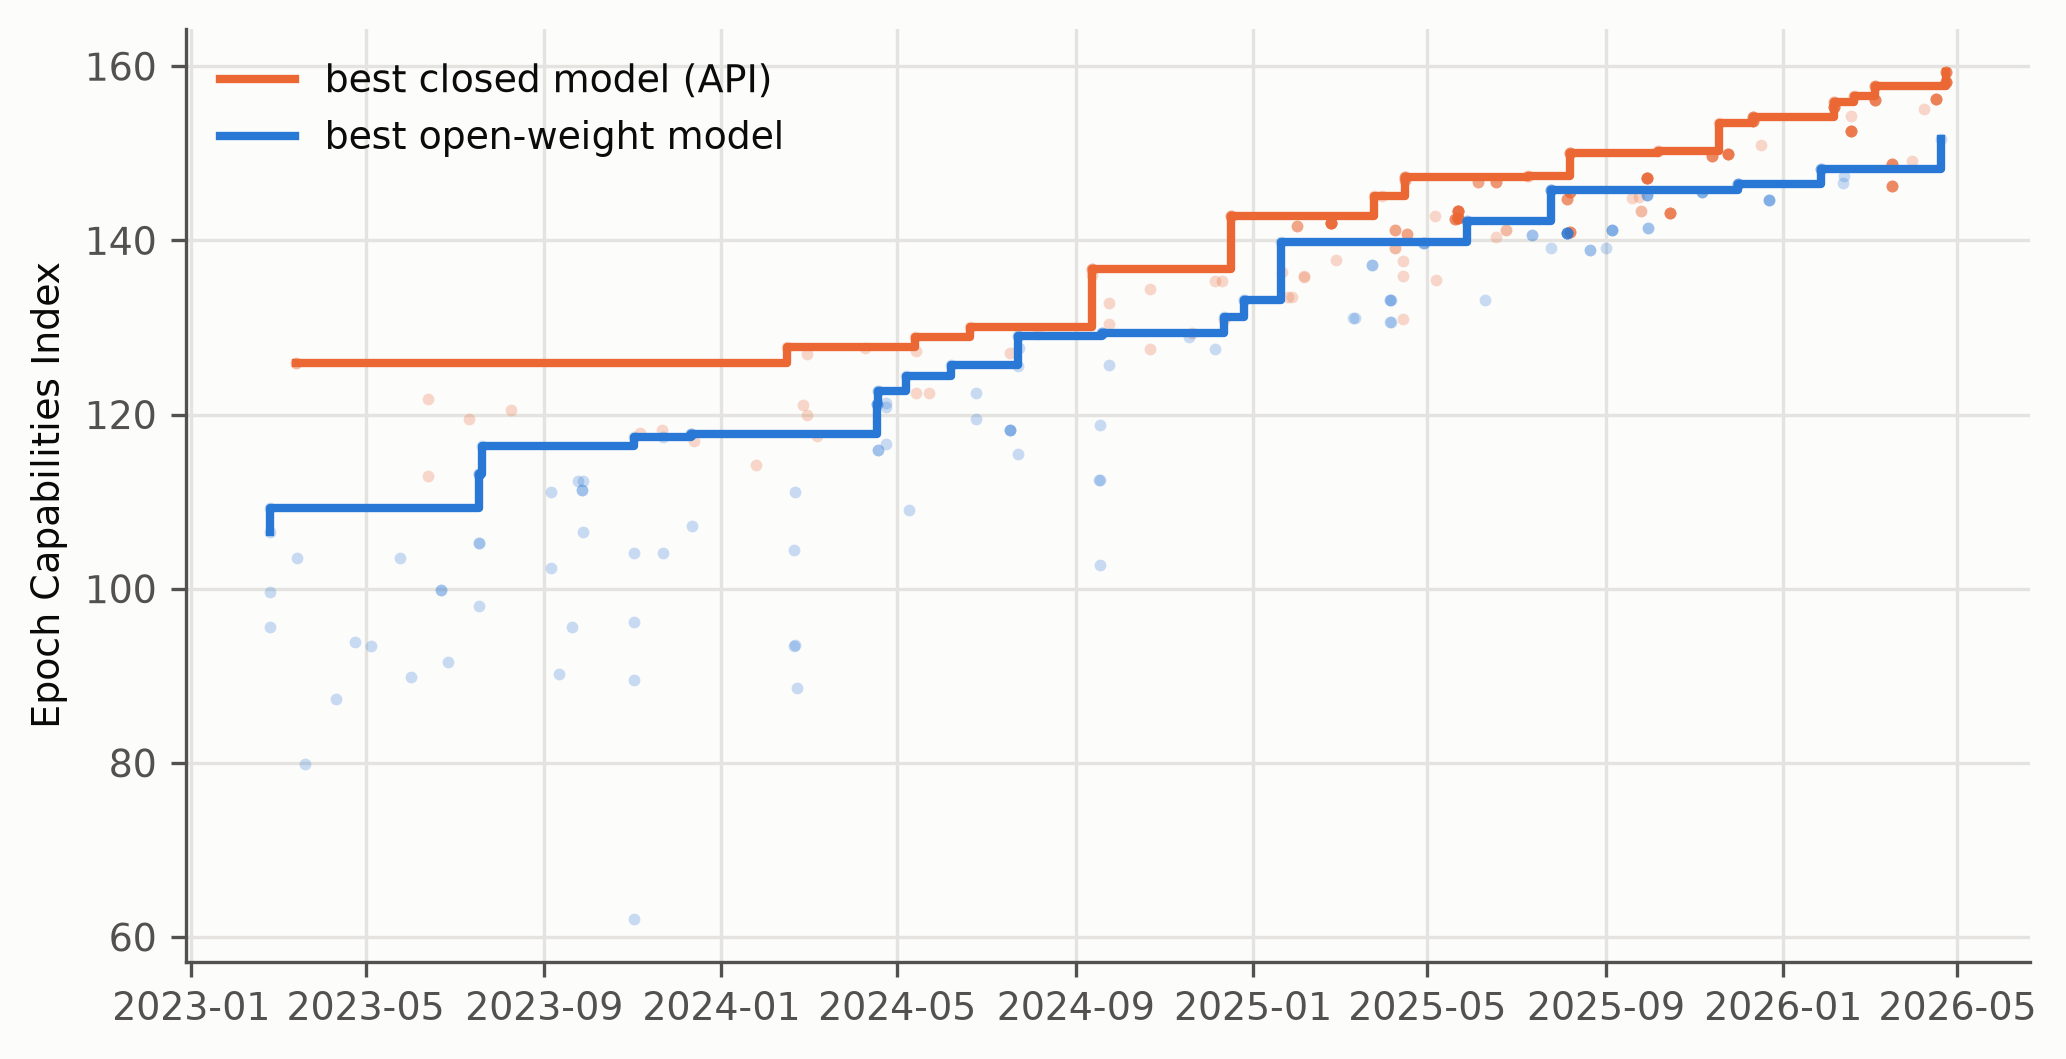
\includegraphics[width=\textwidth]{images/locality/open_closed_gap.png}
\caption{Capability of the best closed and the best open-weight model over time on Epoch AI's aggregate capabilities
index (dots: individual models; lines: best so far). Plotted from Epoch AI's published data table~\cite{epoch2026openclosed}.}
\label{fig:local-gap}
\end{figure}

A more recent snapshot confirms the picture and also shows its limit. On the Artificial Analysis Intelligence Index,
which aggregates ten evaluations, on 20 October 2026 the best closed model, Claude Opus 5.5, scores 58 points, while the
best open-weight model, MiMo-V2.6-Pro, scores 46 (Figure~\ref{fig:local-aa})~\cite{aa2026intelligence}. Several
open-weight models, such as DeepSeek V4.1 Flash, GLM-5.3 and Kimi K3, match or exceed mid-range closed models such as
Claude Haiku 5.5 and Gemini 3.8 Flash. All these open-weight models, however, belong to the class of large models,
whereas the only model in the chart that Artificial Analysis classifies as small, Qwen3.8 27B, stops at 34 points.

This does not mean that large models are excluded from local hardware. The specialised inference engines described in
Section~\ref{sec:local-engines}, such as ds4 and Colibri, run large open-weight models, for example DeepSeek V4 Flash
and GLM-5.2, even when their weights do not fit in memory: they keep the always-active part resident and read the rest
from the SSD. The limit then shifts from capacity to speed. According to the authors of Colibri, GLM-5.2 generates 1.83
tokens per second on a Strix Halo machine with 128\,GB and less than one token per second on a
laptop~\cite{justvugg2026colibri}. For a personal device, therefore, the question is not only which model can be run,
but how fast it can generate text; and generation is precisely the phase that a decision model avoids.

\begin{figure}[htbp]
\centering
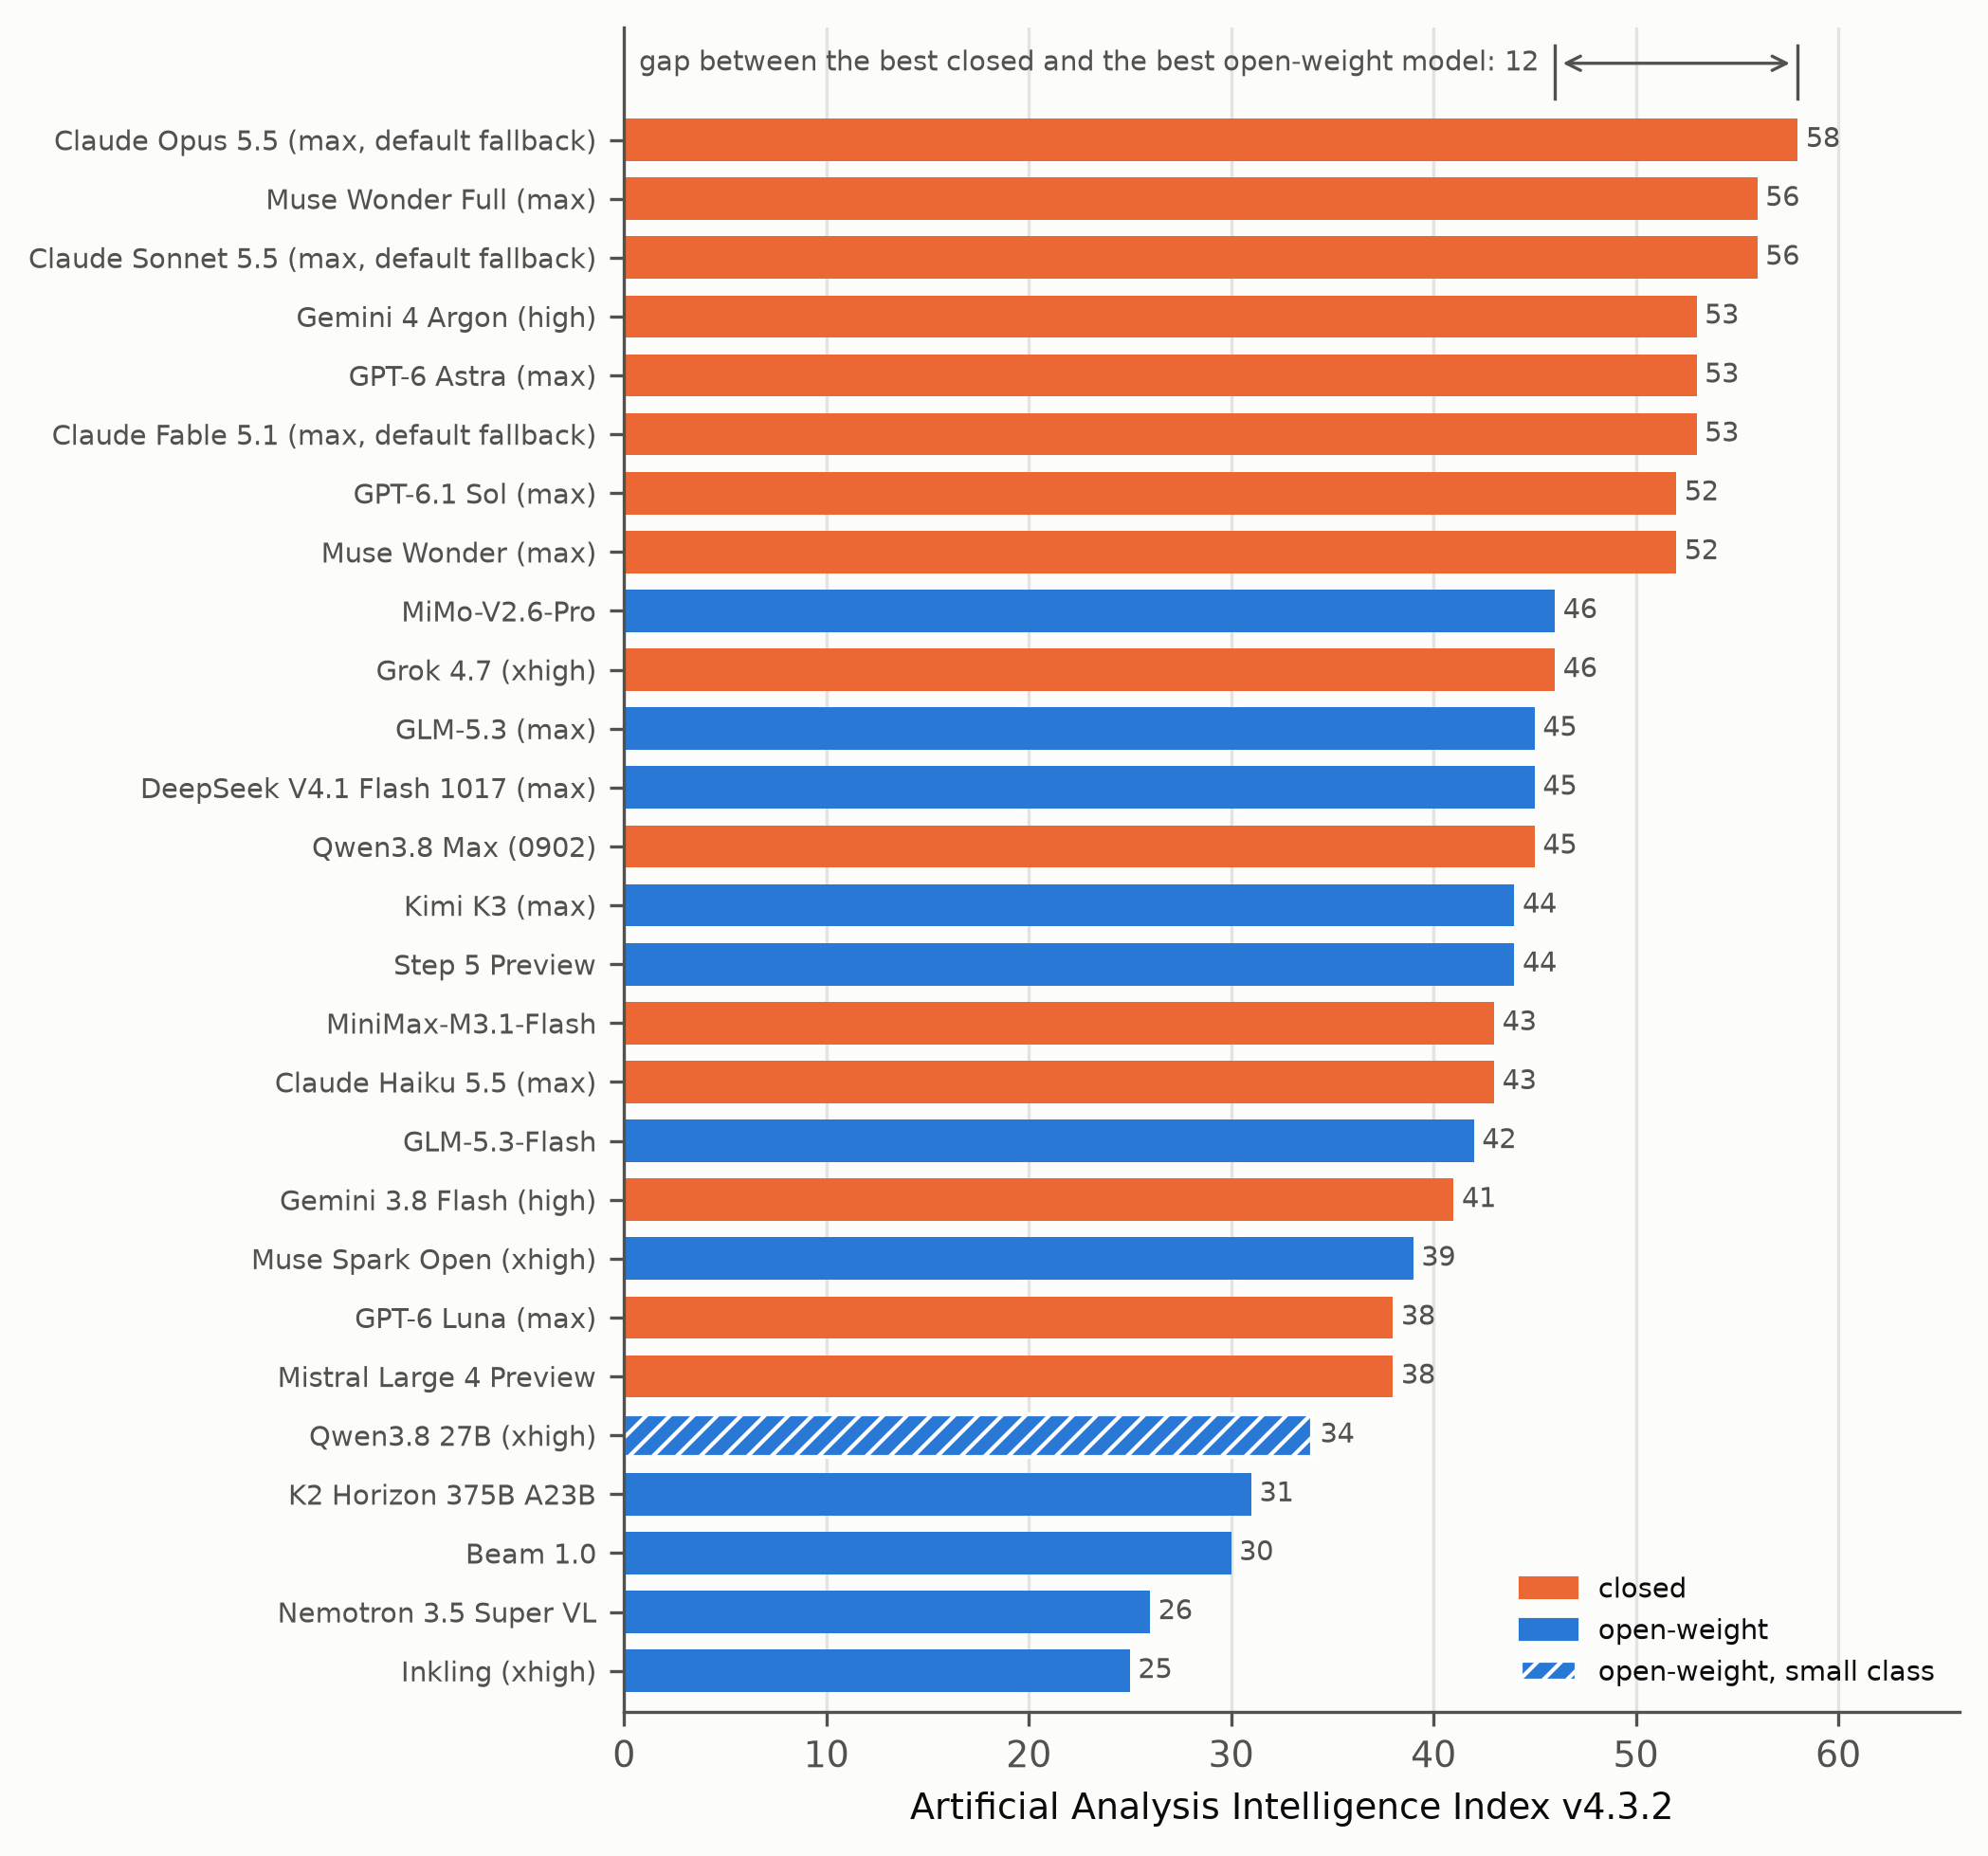
\includegraphics[width=0.92\textwidth]{images/locality/aa_intelligence_snapshot.png}
\caption{Artificial Analysis Intelligence Index (version 4.3.2, ten evaluations) on 20 October 2026, redrawn from the
published chart~\cite{aa2026intelligence}. Closed models in orange, open-weight models in blue; hatched, the only model
that Artificial Analysis classifies as small. In brackets, the reasoning setting at which each model was evaluated. The
open-weight status is taken from the data of the same leaderboard. It is a snapshot: scores and ranking change with
every new release.}
\label{fig:local-aa}
\end{figure}

For interactive use, what matters most is the best model that fits entirely in the memory of consumer hardware, and can
therefore generate without depending on the bandwidth of the SSD. Epoch AI tracks this quantity directly. Considering models small enough to
run on a single consumer graphics card, at most about 28 billion parameters for a card with 24\,GB and about 40 billion
for one with 32\,GB, it finds that across four benchmarks they reach the performance of the frontier model of the time
after six to twelve months~\cite{epoch2025consumergpu}. Three forces drive the catch-up: open-weight developers scale their
training compute about as fast as closed ones, distillation, that is, training a small model to imitate the answers of a
large one, transfers much of its capability, and each new generation of graphics cards raises the size of the models that
fit~\cite{epoch2025bestmodel}. The same trend appears from the other side: the smallest model scoring above 60\,\% on the
MMLU benchmark, a set of multiple-choice questions on 57 subjects, had 540 billion parameters in 2022 and 3.8 billion in 2024, a reduction of 142 times~\cite{stanford2025aiindex}.

\subsection{Small language models}
\label{sec:local-slm}

At the low end of the scale are \emph{small language models}. Definitions vary; a survey that measures several dozen of them on
devices places the range at 100 million to 5 billion parameters, with a decoder-only architecture, that is, the
architecture of common LLMs that generate text from left to right~\cite{lu2024slm}. Small models are trained on far more
data than would be worthwhile if the only aim were to minimise the cost of training. The reason is that, for them, the
cost that matters is inference, repeated millions of times after training: it is therefore worth spending more once to
obtain a small but capable model. A model of half a billion parameters can thus see trillions of
tokens~\cite{lu2024slm}. Measured on edge devices with 4-bit weights, models between 0.1 and 3 billion parameters need
between 0.3 and 2.5\,GB of memory, and at long context most of it is taken by the key-value cache, which stores the
context already read (Section~\ref{sec:local-phases}), and by the computation buffers~\cite{lu2024slm}. Research on models below one billion parameters argues that, on phones, an application should not use
more than about a tenth of the device's memory, and shows that a carefully designed 350-million-parameter model matches a
general 7-billion-parameter model on a narrow task such as calling an application interface~\cite{liu2024mobilellm}.

Platform vendors have adopted the same idea. Apple's foundation model for its devices has about three billion parameters,
is quantised to under four bits per weight and is specialised for each feature with small low-rank adapters, additional
modules with few parameters trained on the single task (Section~\ref{sec:bg-peft})~\cite{gunter2024apple}; Google's Gemma~3n family is designed to run on phones and laptops with a reduced memory
footprint, and is marketed explicitly for privacy and offline use~\cite{google2025gemma3n}. GroundOne follows the same
pattern: a small open-weight model, quantised, specialised by an adapter for one task.

\section{The cost of inference on one device}
\label{sec:bg-inference}

The previous sections explain why a model should run locally and which models can. This section explains how much it
costs to run one, and why the cost depends so strongly on what the model is asked to do.

\subsection{Prefill and decode}
\label{sec:local-phases}

A decoder-only language model processes a request in two phases. In the \emph{prefill} phase it reads the whole prompt at
once. To do so it uses the attention mechanism, through which each token gathers information from the tokens that
precede it: every layer computes, for each input token, two vectors (a \emph{key} and a \emph{value}) that later tokens
will consult, and stores them in the \emph{key-value cache}. In the \emph{decode} phase it produces the output
one token at a time; each new token consults the cache through attention and extends it by one
position~\cite{pope2023scaling}. Prefill processes many tokens in parallel; decoding
processes one. Serving systems exploit the difference in several ways, for instance by managing the cache in pages to fit
more concurrent requests~\cite{kwon2023pagedattention} or by running the two phases on different machines suited to
each~\cite{patel2024splitwise}.

The consequence is visible on the laptop used in this thesis (Figure~\ref{fig:local-prefill-decode}). With the 0.5B model,
reading one token of the prompt takes less than 0.4 milliseconds, while writing one token of output takes 5.9 milliseconds,
sixteen times more. With the 3B model the figures are 2.2 and 31.8 milliseconds, fourteen times more. A model that writes a
short paragraph thus spends more time on it than on reading a document of several thousand tokens.

\begin{figure}[htbp]
\centering
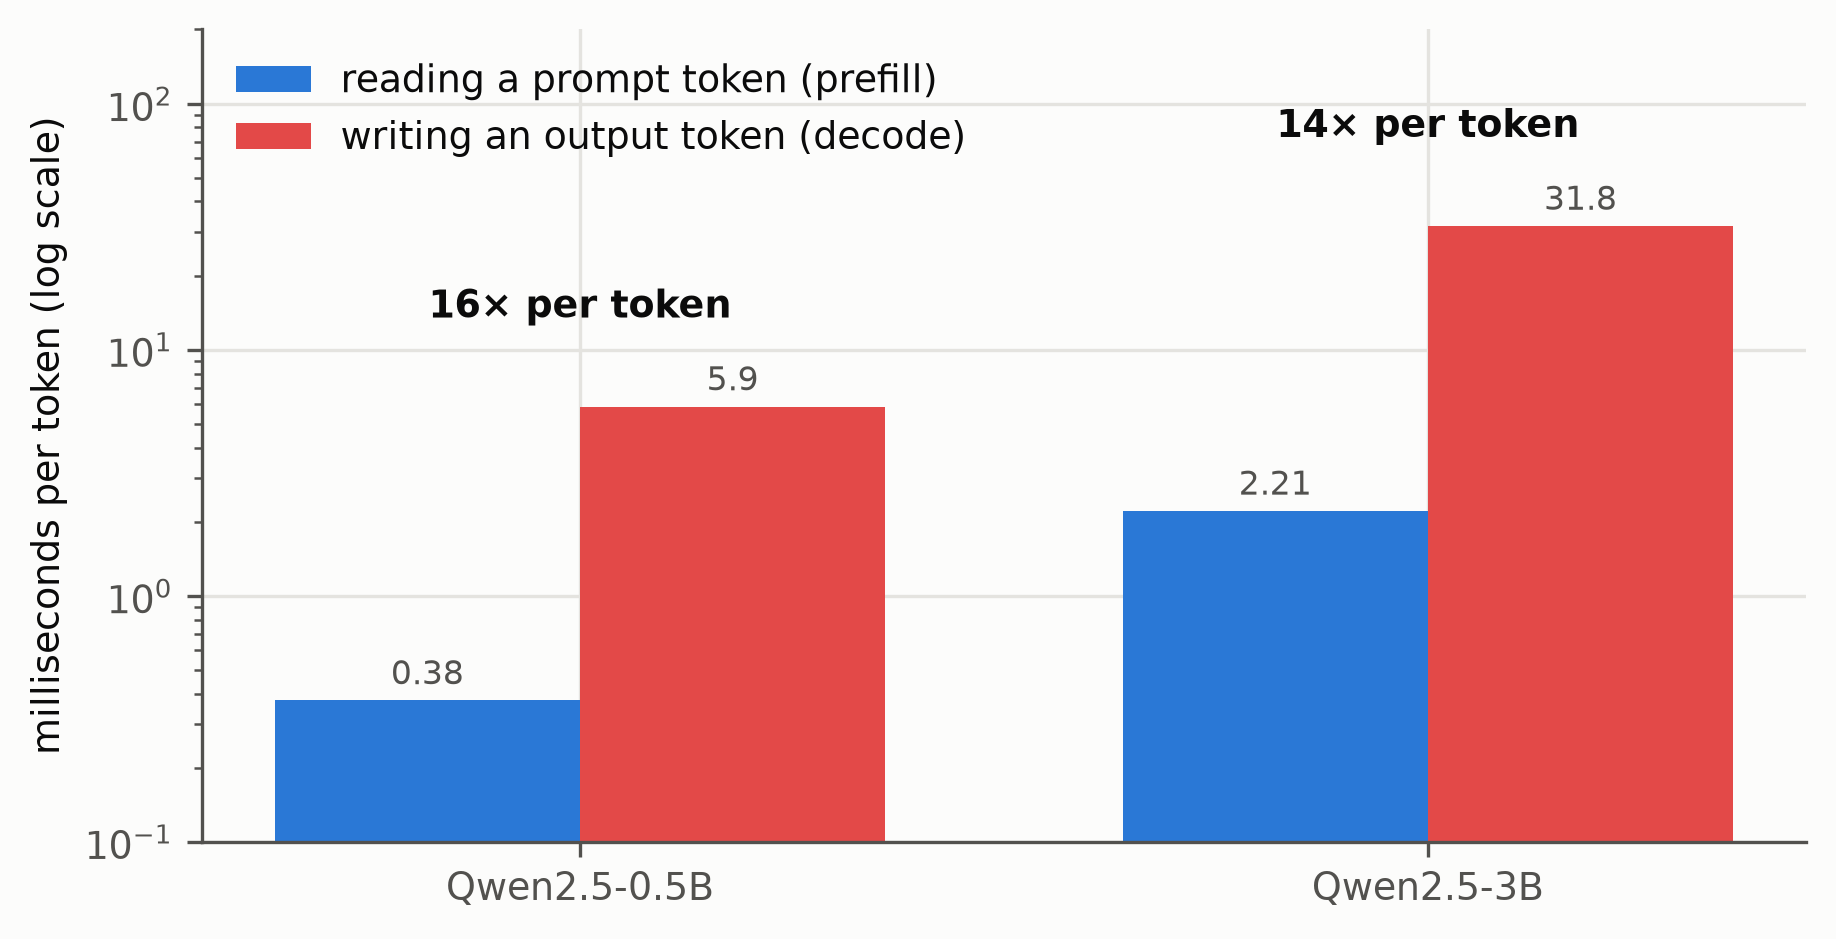
\includegraphics[width=0.85\textwidth]{images/locality/prefill_vs_decode_m4.png}
\caption{Time per token when the model reads its input (prefill) and when it writes its output (decode), measured on the
thesis machine (Apple M4, 16\,GB, MLX 8-bit, one request at a time). Prefill: median over contexts of 500, 1,000 and 2,000 tokens.}
\label{fig:local-prefill-decode}
\end{figure}

\subsection{The roofline model}
\label{sec:local-roofline}

The reason for this asymmetry is captured by the roofline model, a simple model of performance introduced for multicore
processors~\cite{williams2009roofline}. A computation is characterised by its \emph{arithmetic intensity}, the number of
floating-point operations it performs for each byte it reads from memory. A processor has two limits: a peak rate of
computation and a peak memory bandwidth. The attainable rate is the minimum of the peak computation and the product of
bandwidth and intensity. A computation with low intensity is limited by the bandwidth, and one with high intensity by the
computation; the intensity at which the two limits meet is called the ridge point~\cite{williams2009roofline}.

Applied to a transformer, the model separates the two phases cleanly~\cite{yuan2024unveiled}. Each weight matrix of a
linear layer must be read from memory once per forward pass. During prefill the same matrix multiplies the hidden states
of hundreds or thousands of tokens, so each byte of weights is used for hundreds of operations: the intensity is high and
the computation is the limit. During decoding, the matrix multiplies a single vector, so each weight is used for about
two operations: the intensity is close to one and the bandwidth is the limit. For a 7-billion-parameter model in 16-bit
precision, the linear layers reach intensities above one thousand operations per byte in prefill and about one in
decode~\cite{yuan2024unveiled}. In datacenters this imbalance is softened: the decoding of many concurrent requests is
grouped into batches, so that each weight read from memory serves to generate several tokens and the intensity
rises~\cite{pope2023scaling}. A personal device serves a single user, one request at a time, and cannot rely on this
remedy: this is where the asymmetry between the two phases weighs most.

Figure~\ref{fig:local-roofline} draws the roofline of the thesis machine. Apple publishes its memory bandwidth, 120\,GB/s,
but no peak rate of computation~\cite{apple2024m4specs}; the flat roof in the figure is therefore the rate actually reached
during prefill, about 2.8 TFLOP/s, which is a lower bound of the peak. The ridge point lies at about 23
operations per byte. Generating a token sits at about two operations per byte, an order of magnitude below the ridge,
whereas reading a document of hundreds of tokens sits an order of magnitude above it. The two phases of the same model,
on the same machine, live in different regimes.

\begin{figure}[htbp]
\centering
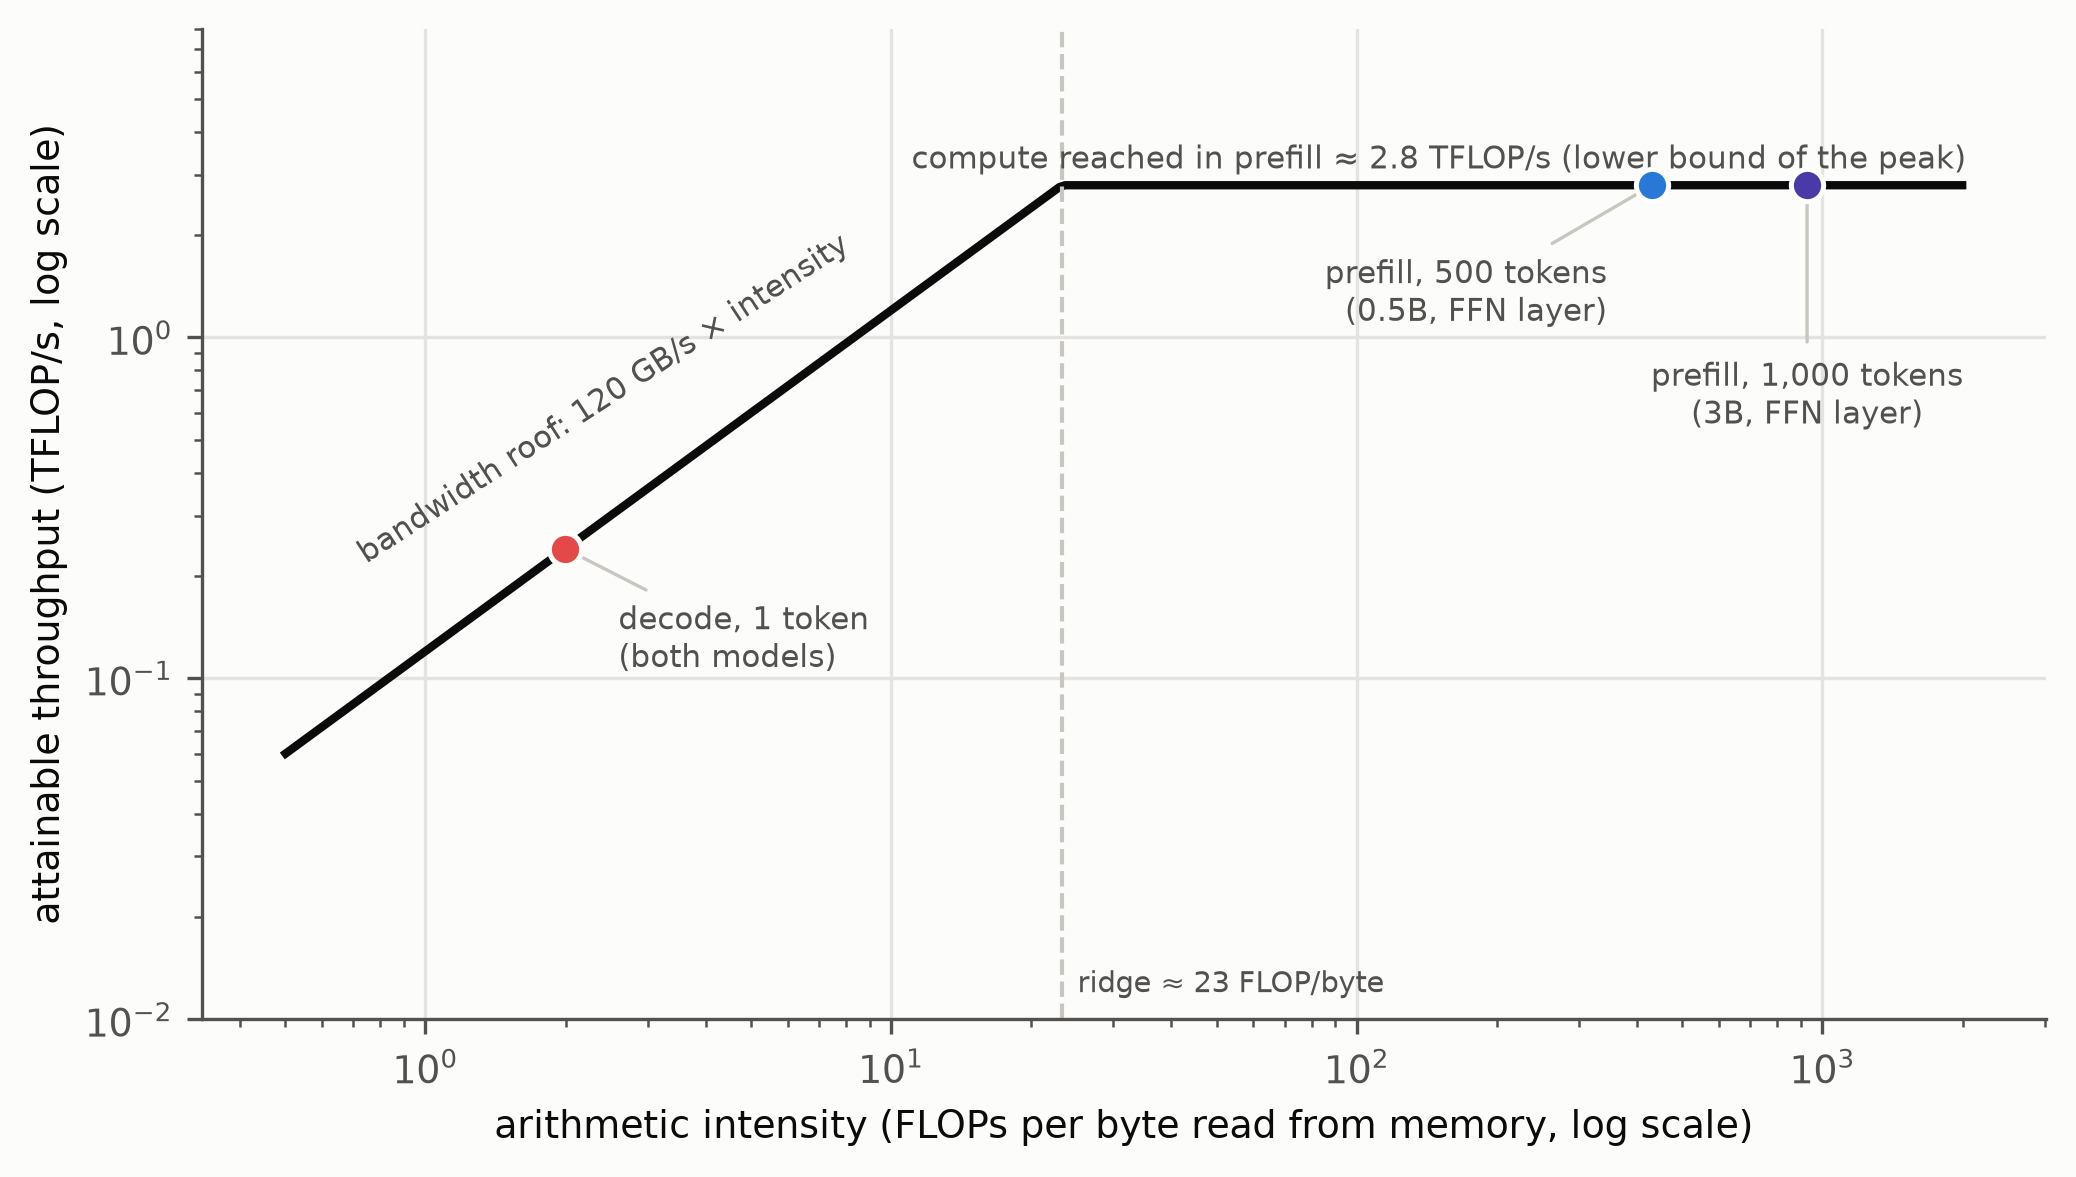
\includegraphics[width=\textwidth]{images/locality/roofline_m4.png}
\caption{Roofline model of the thesis machine~\cite{williams2009roofline}. Sloped roof: Apple's memory bandwidth (120\,GB/s).
Flat roof: throughput reached in prefill, a lower bound of the unpublished peak. Intensities computed for one feed-forward
layer of Qwen2.5 with 8-bit weights and 16-bit activations; attention is ignored.}
\label{fig:local-roofline}
\end{figure}

\subsection{A lower bound on generation}
\label{sec:local-floor}

Because decoding reads every weight once per generated token, its time per token cannot be lower than the size of the
weights divided by the memory bandwidth, whatever the hardware. For the 3B model in 8-bit precision, whose weights occupy
about 3.3\,GB, this floor is 27 milliseconds per token on a machine with 120\,GB/s; the measured 31.8 milliseconds are
only about one sixth above it. The bound depends only on two numbers, the size of the model and the bandwidth of the machine, and
it applies to every model that generates text. It is the key to comparing hardware in Section~\ref{sec:local-hardware}
and to the consequence drawn in Section~\ref{sec:local-verification}.

Memory capacity sets a second, harder limit: the weights must fit. A model needs about two bytes per parameter in the
16-bit format used for training, one in 8 bits and half in 4 bits, plus a few small scale factors for each group of
weights, needed to reconstruct their values (Figure~\ref{fig:local-memory}). A 7-billion-parameter model in 16 bits needs 14\,GB for its weights alone, beyond what most
personal devices can spare~\cite{alizadeh2024flash}; in 4 bits it needs about 4\,GB. The key-value cache, the activations,
the operating system and every other model that runs at the same time come on top. A laptop with 16\,GB can therefore
hold a generator of 7--8 billion parameters in 4 bits next to a small verifier, but not much more.

\begin{figure}[htbp]
\centering
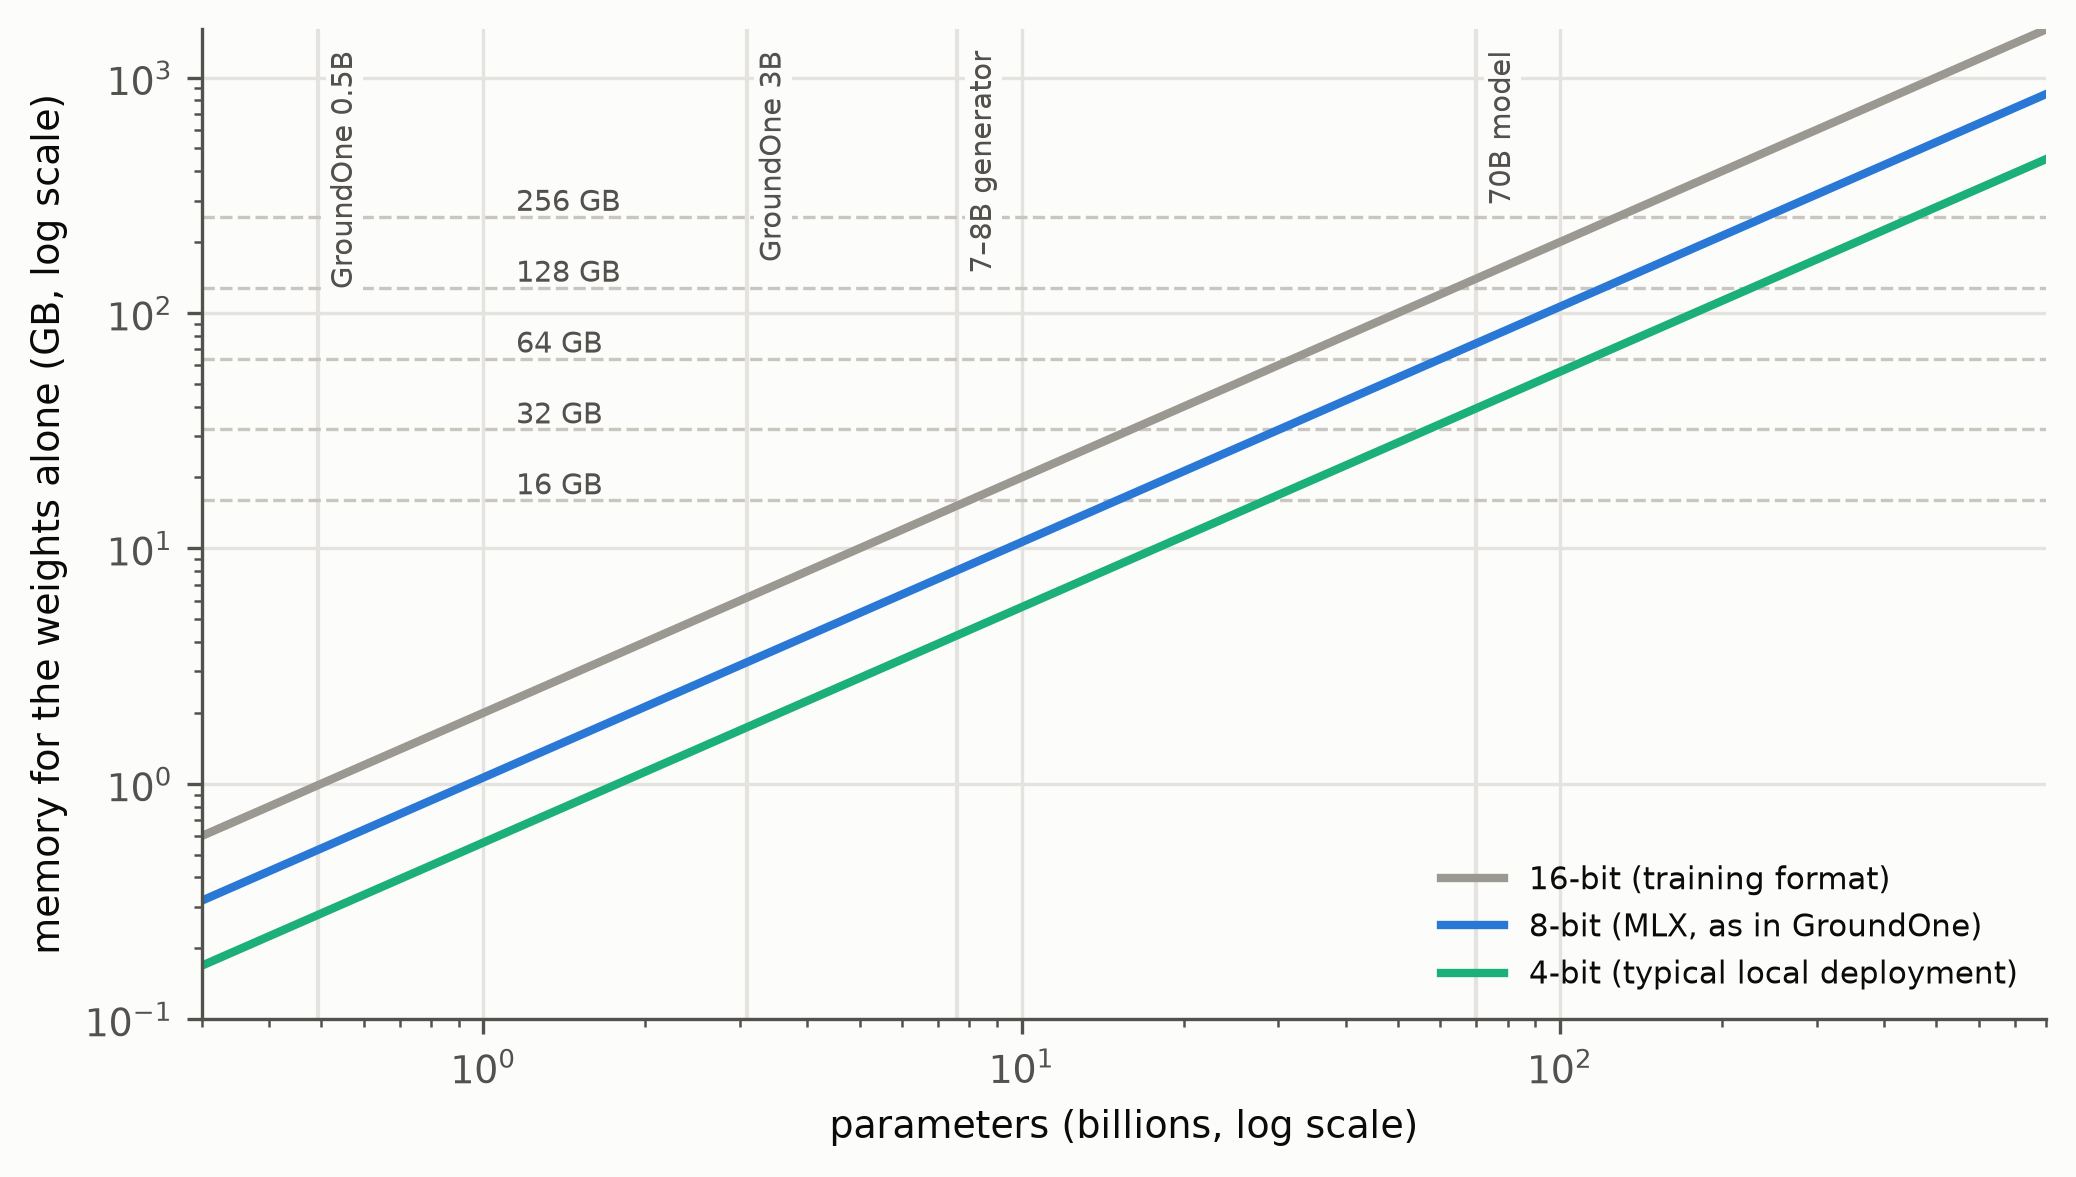
\includegraphics[width=\textwidth]{images/locality/memory_fit.png}
\caption{Memory needed for the weights of a model as a function of its size and precision (parameters times bits per
weight, including half a bit of per-group scales for the quantised formats). Dashed lines: common memory sizes of local
hardware. The key-value cache, activations and other running models come on top.}
\label{fig:local-memory}
\end{figure}

\section{Hardware for local inference}
\label{sec:local-hardware}

The cost model reduces the choice of hardware for local inference to three quantities. \emph{Memory capacity} decides
which models fit. \emph{Memory bandwidth} decides how fast they can generate. \emph{Computation} decides how fast they can
read. Power and price complete the picture. This section surveys the hardware available in October 2026 along these axes,
using the vendors' published specifications.

\subsection{Classes of hardware}
\label{sec:local-classes}

Two architectures dominate. In a \emph{discrete} system, the graphics card has its own memory, fast but small, and the
model must fit in it. In a \emph{unified-memory} system, the processor and the graphics unit share one large pool of
memory, so a model can use most of the machine's memory, at a lower bandwidth than a high-end graphics card. Apple's
processors, NVIDIA's DGX Spark and AMD's Ryzen AI Max (Strix Halo) all follow the second design. Figure~\ref{fig:local-memarch} compares the two architectures.

\begin{figure}[htbp]
\centering
\subfloat[Discrete system: the GPU reads the weights from its own VRAM, very fast but limited to 16--32\,GB; the rest of
the system is reachable only through PCIe.]{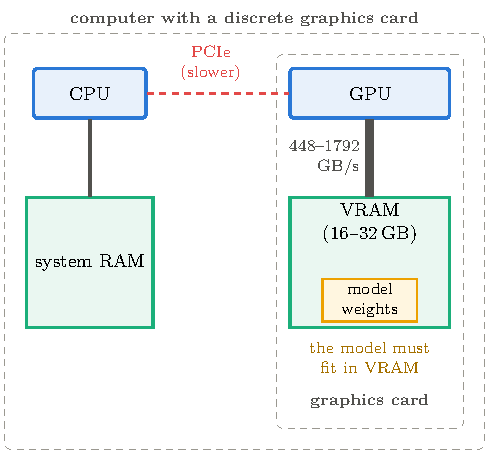
\includegraphics[width=0.53\textwidth]{images/diagrams/memory_discrete_tikz.pdf}\label{fig:local-memarch-discrete}}\hfill
\subfloat[Unified memory: CPU, GPU and NPU on the same chip share one pool of memory, larger but with lower
bandwidth.]{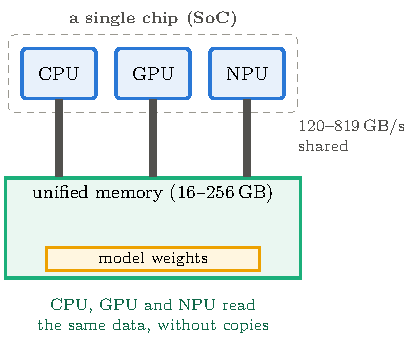
\includegraphics[width=0.43\textwidth]{images/diagrams/memory_unified_tikz.pdf}\label{fig:local-memarch-unified}}
\caption{The two architectures of local inference hardware. Blue rectangles: compute units; green rectangles: memory;
orange rectangle: the model weights; line width: indicative bandwidth. Capacity and bandwidth values from
Table~\ref{tab:local-hardware}. In a discrete system a model that does not fit in VRAM must go through the much slower
PCIe link; in a unified-memory system the model can occupy almost all of the machine's memory, but every generated token
reads it at a lower speed than a high-end graphics card.}
\label{fig:local-memarch}
\end{figure}
Table~\ref{tab:local-hardware} and Figure~\ref{fig:local-hardware} place the main options on the two memory axes. Figure~\ref{fig:local-photos} shows some of the
systems discussed, to give a concrete idea of what they look like.

\begin{figure}[htbp]
\centering
\subfloat[14-inch MacBook Pro with M4, the thesis machine.]{
\includegraphics[width=0.31\textwidth]{images/hardware/macbook_pro_m4.png}}\hfill
\subfloat[Mac mini (2024, M4).]{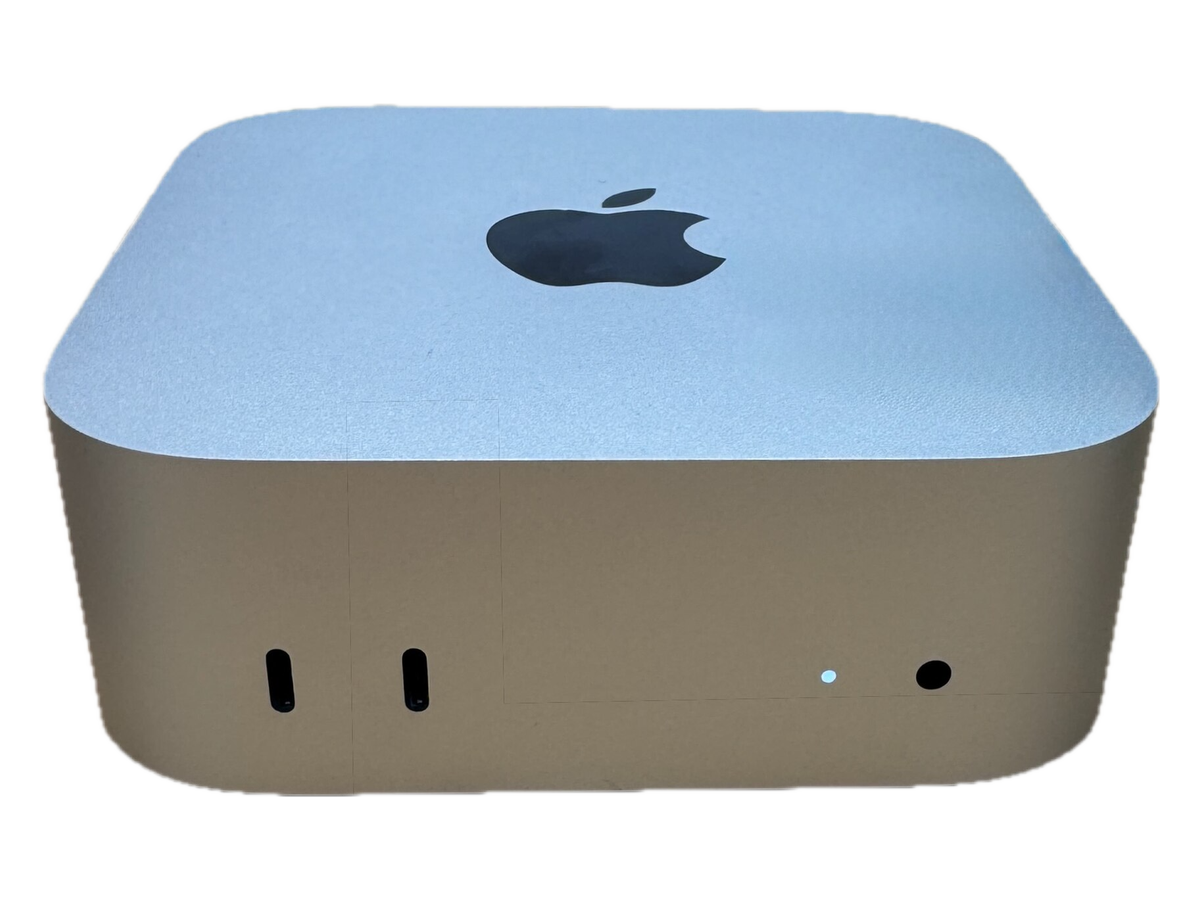
\includegraphics[width=0.31\textwidth]{images/hardware/mac_mini_m4.png}}\hfill
\subfloat[Mac Studio.]{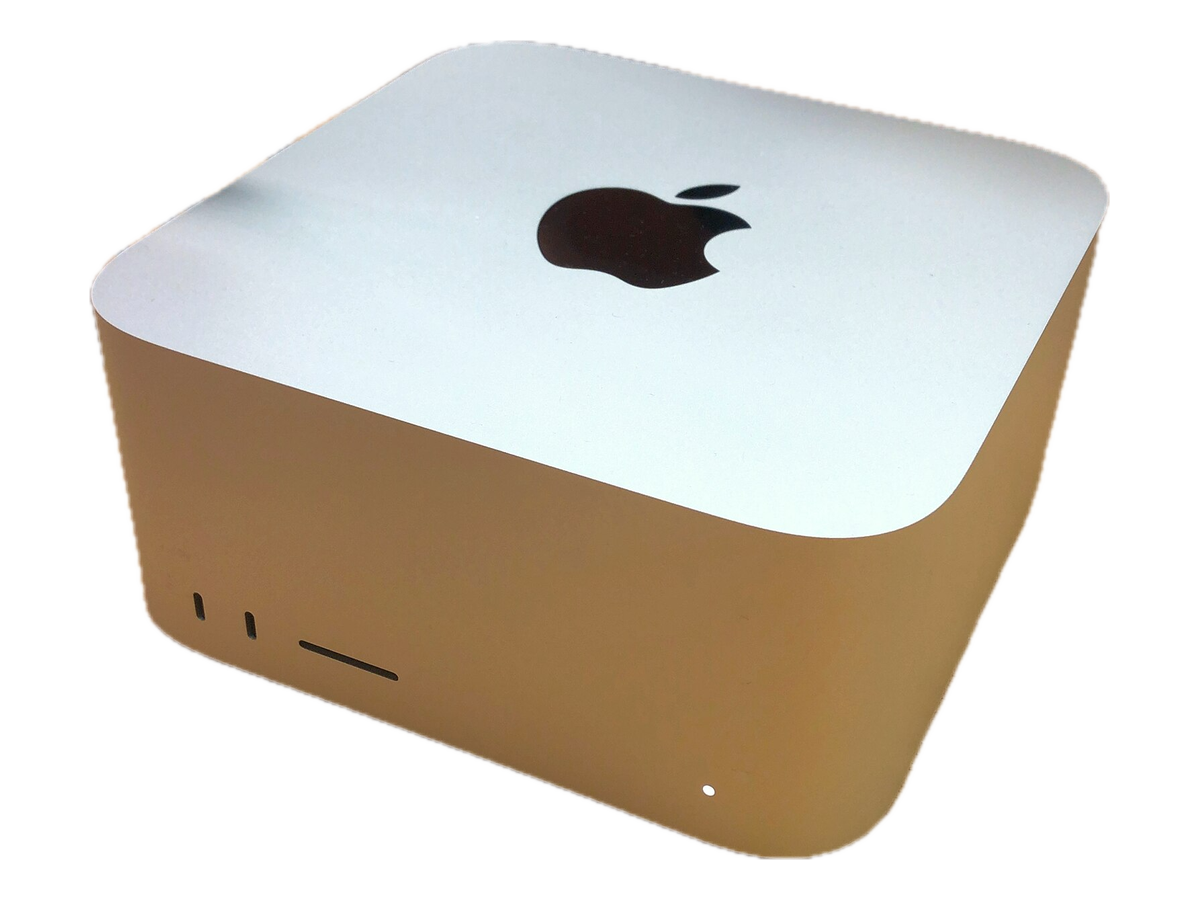
\includegraphics[width=0.31\textwidth]{images/hardware/mac_studio.png}}\\[0.6em]
\subfloat[NVIDIA DGX Spark.]{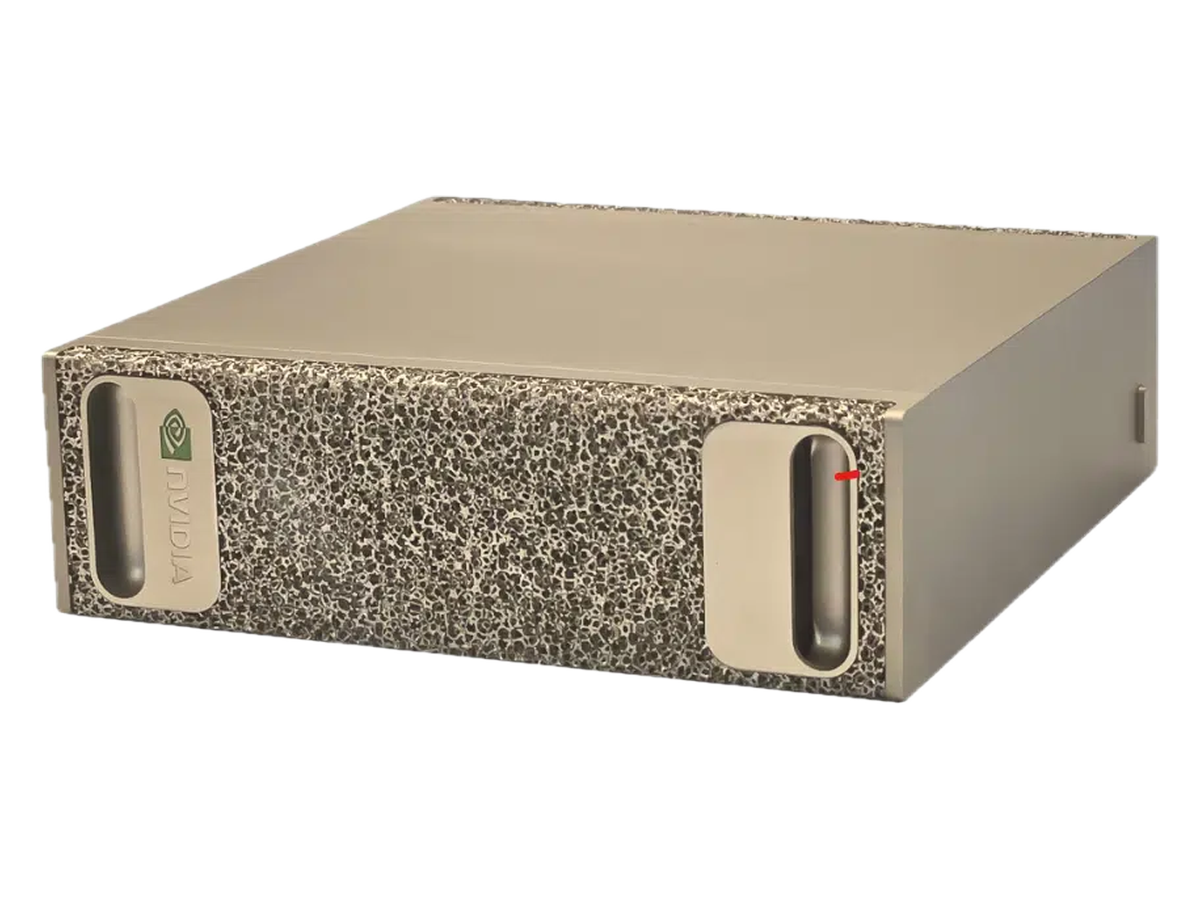
\includegraphics[width=0.31\textwidth]{images/hardware/dgx_spark.png}}\hspace{0.035\textwidth}
\subfloat[GeForce RTX 5090 Founders Edition graphics card.]{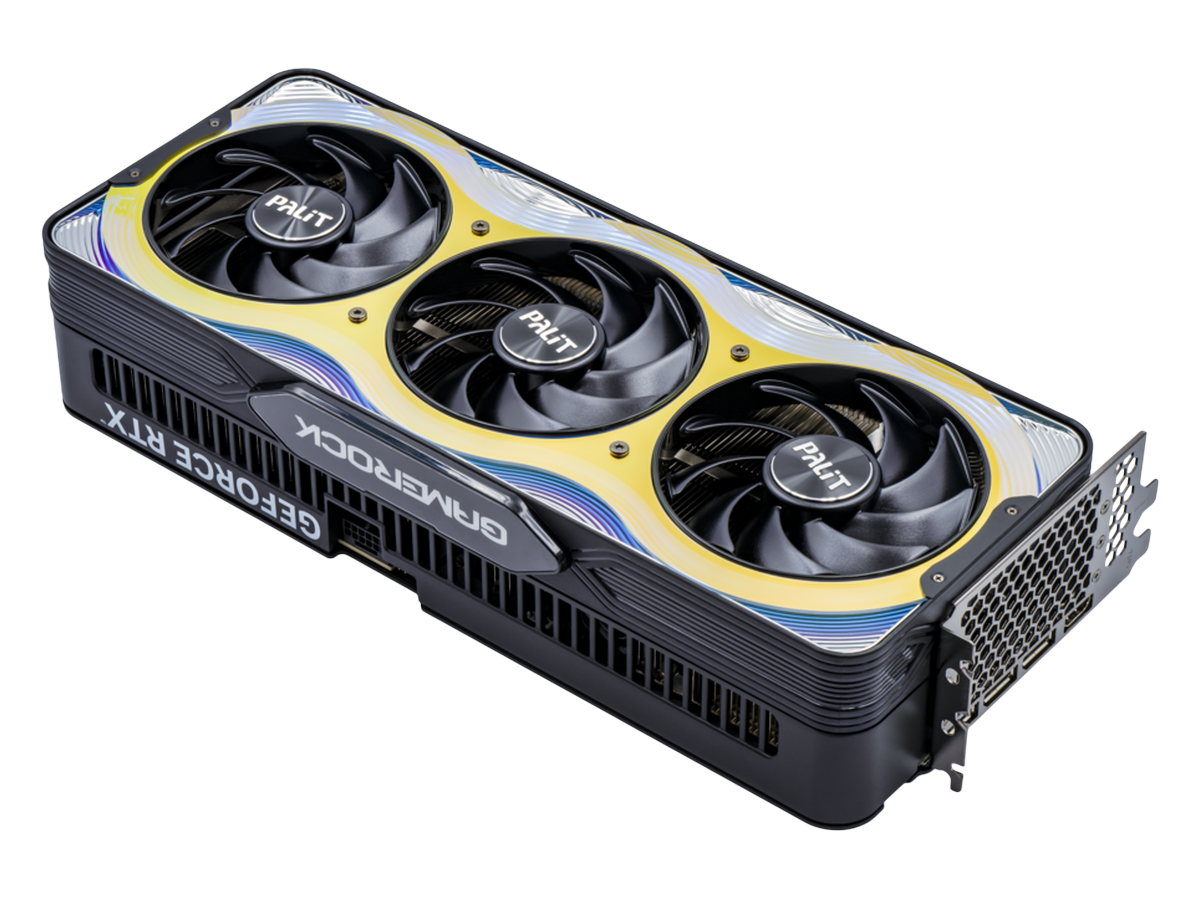
\includegraphics[width=0.31\textwidth]{images/hardware/rtx_5090.png}}
\caption{Some of the local inference systems compared in this section (images not to scale). Sources: (a), (c) Apple;
(b) LoMit, Wikimedia Commons, CC0; (d), (e) NVIDIA. The vendors' images are promotional material, reproduced for the
purpose of scientific documentation.}
\label{fig:local-photos}
\end{figure}

\begin{table}[htbp]
\centering
\caption{Hardware for local inference: vendors' published specifications (accessed 2026-10-11). Memory: range of the
configurations offered; bandwidth: for those configurations; n/s: not stated by the source.}
\label{tab:local-hardware}
\small
\begin{tabularx}{\textwidth}{@{}Xrrll@{}}
\toprule
System & Memory (GB) & Bandwidth (GB/s) & Memory type & Source \\
\midrule
MacBook Pro, M4 (thesis machine: 16\,GB) & 16--32 & 120 & Unified & \cite{apple2024m4specs} \\
MacBook Pro / Mac mini, M5 & 16--32 & 153 & Unified & \cite{apple2026mbp,apple2026macmini} \\
Mac mini, M5 Pro & 24--64 & 307 & Unified & \cite{apple2026macmini} \\
MacBook Pro, M5 Max & 36--128 & 460--614 & Unified & \cite{apple2026mbp} \\
Mac Studio, M4 Max & 36--128 & 410--546 & Unified & \cite{apple2025macstudio} \\
Mac Studio, M3 Ultra & 96--256 & 819 & Unified & \cite{apple2025macstudio} \\
NVIDIA DGX Spark (GB10) & 128 & 273 & Unified & \cite{nvidia2026dgxspark} \\
Framework Desktop, AMD Strix Halo & 32--128 (96 to GPU) & n/s & Unified & \cite{hachman2025framework} \\
NVIDIA RTX 5090 & 32 & 1,792 & Discrete & \cite{nvidia2026geforce} \\
NVIDIA RTX 5080 & 16 & 960 & Discrete & \cite{nvidia2026geforce} \\
NVIDIA RTX 5060 Ti & 16 & 448 & Discrete & \cite{nvidia2026geforce} \\
\bottomrule
\end{tabularx}
\end{table}

\begin{figure}[htbp]
\centering
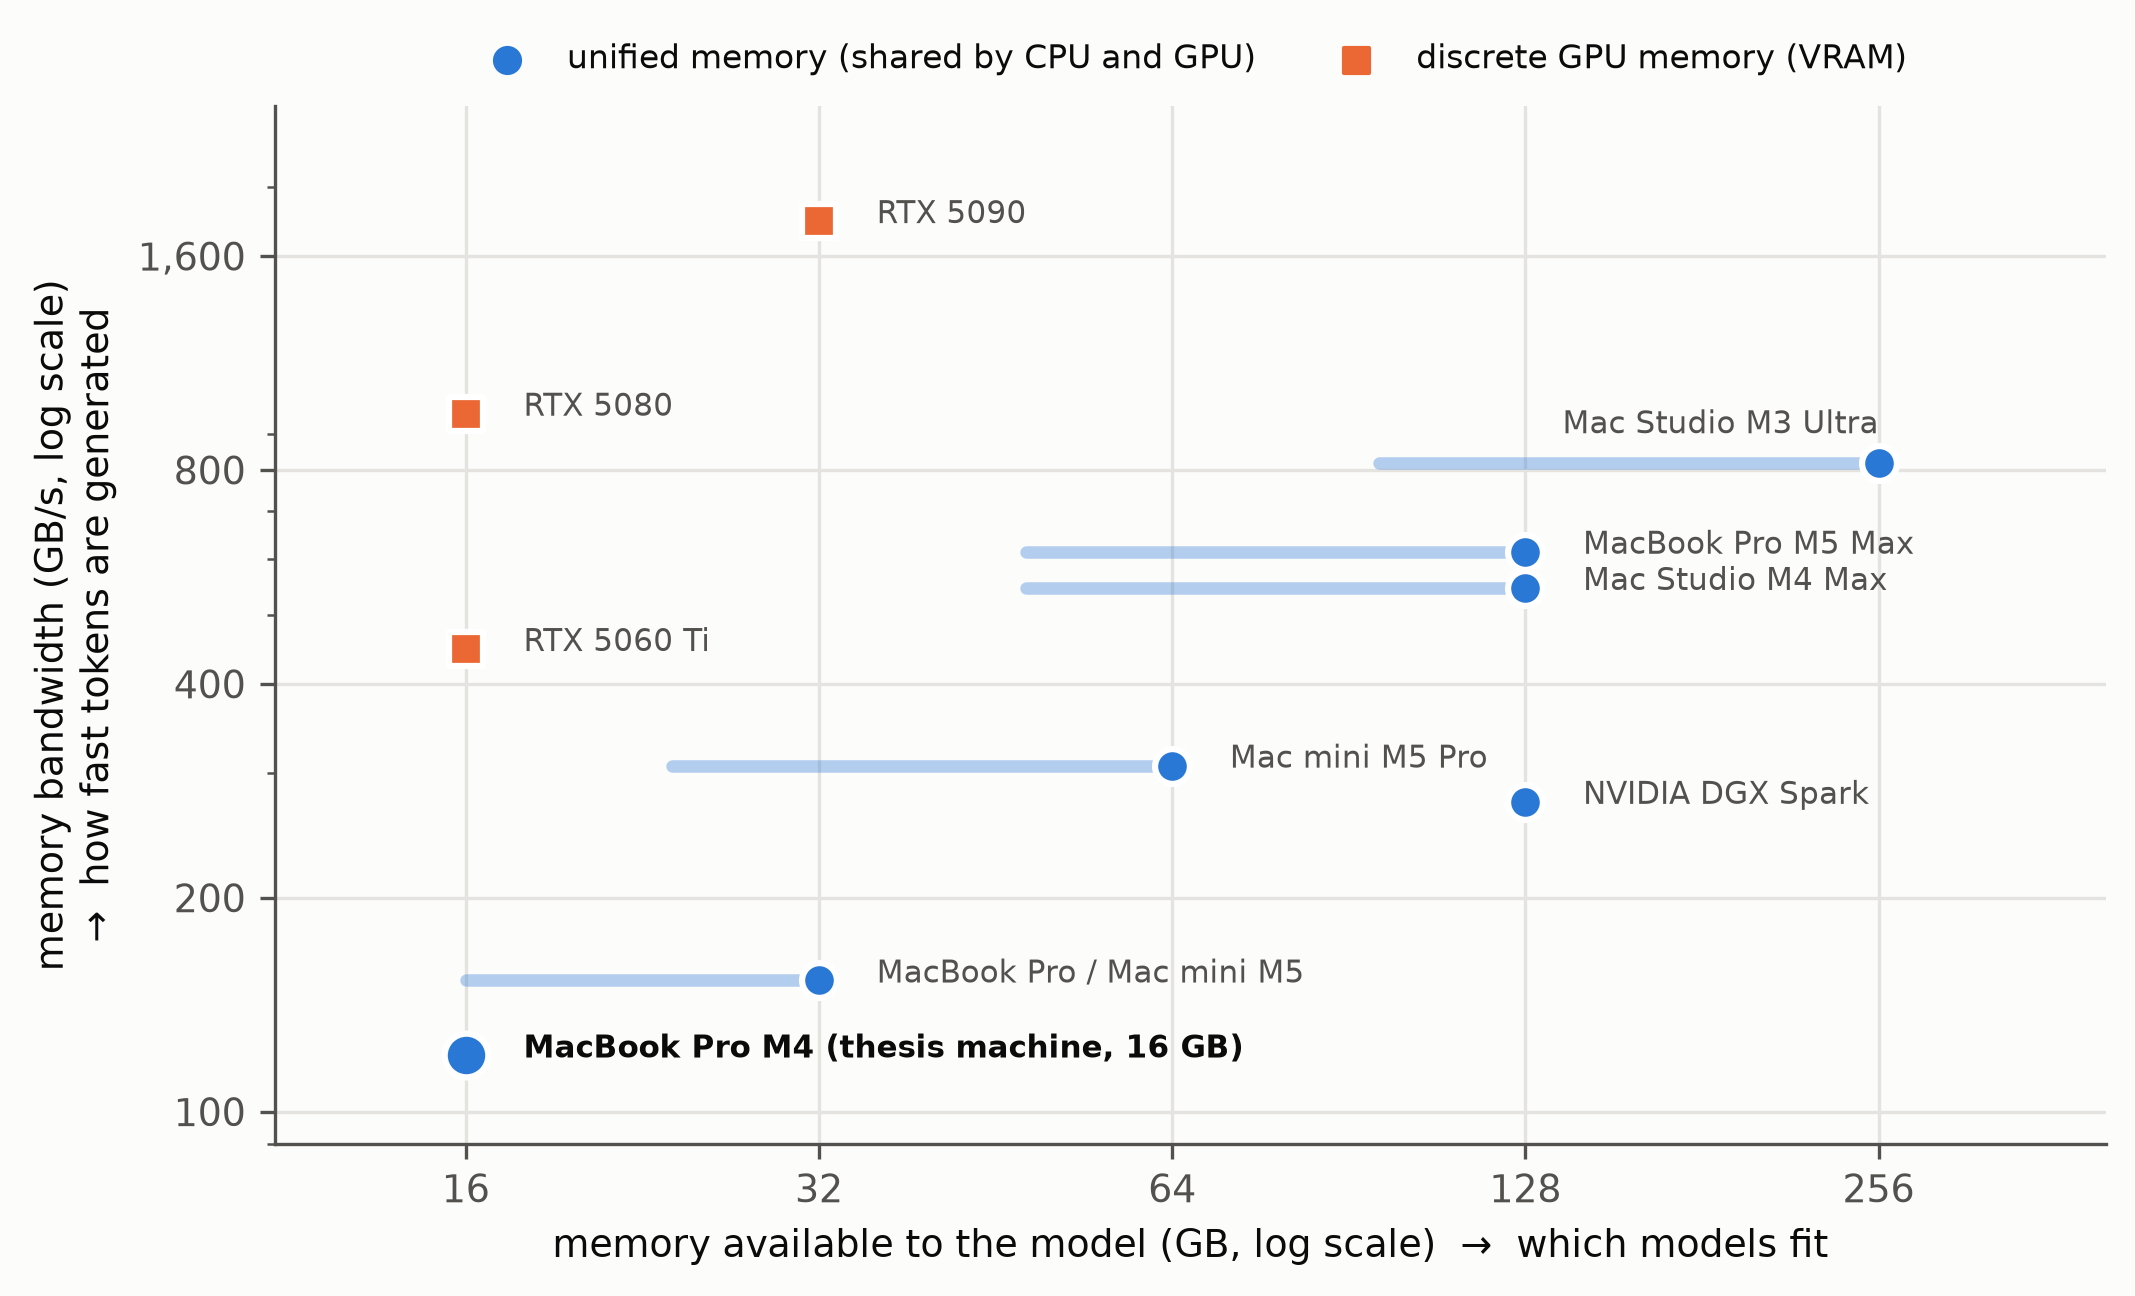
\includegraphics[width=\textwidth]{images/locality/hardware_landscape.png}
\caption{Local inference hardware on the two axes that decide what can run: memory capacity (which models fit) and memory
bandwidth (how fast tokens are generated). Vendors' specifications: markers at the largest memory configuration, shaded
bars over the range of memory sizes offered; the thesis machine is shown at its actual 16\,GB.}
\label{fig:local-hardware}
\end{figure}

\paragraph{Laptops.} Laptops with 16 to 32\,GB and 120 to 150\,GB/s, such as the MacBook Pro used in this thesis, are the
most common personal computers on which local models run. They hold small models comfortably and models of 7--8 billion
parameters in 4 bits. The thesis machine sits at the bottom left of Figure~\ref{fig:local-hardware}: if a verifier runs
well there, it runs on everything above it.

\paragraph{Desktop machines with unified memory.} A second class, within or close to a budget of about three thousand
dollars, offers much more memory at moderate bandwidth. AMD's Strix Halo processor, sold for instance in the Framework
Desktop, lets the graphics unit use up to 96\,GB of its 128\,GB of memory; the 128\,GB configuration was priced at
1,999 dollars at launch in August 2025, with a processor power of 55\,W~\cite{hachman2025framework}. Apple's Mac mini with
the M5 Pro reaches 64\,GB at 307\,GB/s~\cite{apple2026macmini}. Such machines can hold models of tens of billions of
parameters or mixture-of-experts models, which are composed of many sub-networks (the experts) of which each token
activates only a part, so that decoding reads only the weights of the active experts, at the price of a slower
generation than on a graphics card.

\paragraph{Dedicated AI machines.} Above this budget, the Mac Studio with the M3 Ultra combines up to 256\,GB with
819\,GB/s~\cite{apple2025macstudio}, whereas NVIDIA's DGX Spark is a small desktop box, with a 240\,W power supply, that
contains 128\,GB of unified memory with 273\,GB/s of bandwidth and a Blackwell graphics unit rated at one petaflop
($10^{15}$ operations per second) in 4-bit arithmetic, a figure that exploits sparsity, that is, the skipping of zero
weights~\cite{nvidia2026dgxspark}. The two machines make opposite choices, and a direct comparison shows the cost model at
work: on an 8-billion-parameter model with an 8,000-token prompt, the DGX Spark completes the prefill 3.8 times faster
than the Mac Studio, thanks to its higher computation, while the Mac Studio generates 3.4 times faster, thanks to its
three times higher bandwidth~\cite{exo2025spark}. The same study combines the two machines, running the prefill on the
Spark and the decoding on the Mac, which is the disaggregation of the two phases~\cite{patel2024splitwise} brought to a
desk.

\paragraph{Graphics cards.} Discrete cards offer by far the highest bandwidth, up to 1,792\,GB/s for the RTX 5090, but at
most 32\,GB of memory, at a power of several hundred watts~\cite{nvidia2026geforce}. They are the fastest option for any
model that fits, and unusable for any model that does not.

\paragraph{Phones and mobile processors.} At the other end, phones have 6 to 16\,GB of memory and a bandwidth of a few
tens of gigabytes per second shared by all processors~\cite{li2025collaborative,xue2024powerinfer2}. Their neural
processing units (NPUs) are fast at 8-bit matrix multiplication and therefore at prefill: on a phone, a
7-billion-parameter model in 4 bits reads its prompt at about 770 tokens per second on the NPU, against 37 on the
graphics unit and 8 on the processor cores~\cite{xue2024powerinfer2}. Research systems exploit this by running the
prefill on the NPU and the decoding elsewhere~\cite{xu2025npu}.

\subsection{The asymmetry holds on every class}
\label{sec:local-asymmetry}

The two phases respond to different properties of the hardware, and recent hardware generations make the point
explicit. Apple reports that its M5 processor, which adds dedicated matrix units to each graphics core, reduces the time
to first token, that is, the wait before the model starts answering, which is dominated by prefill, by 3.3 to 4.1 times with respect to the M4, while generation becomes
only 1.19 to 1.27 times faster, in line with a memory bandwidth that grew from 120 to 153\,GB/s~\cite{apple2025m5mlx}.
Apple itself attributes the first figure to computation and the second to bandwidth. On edge devices, a study that
compares 18 pairs of configurations finds that slowdowns accumulate in decoding, while the time to evaluate the prompt
changes by at most 16\,\%~\cite{das2026edge}. On phones, for tasks whose output is short, prefill takes most of the
latency~\cite{xu2025npu}. Hardware is thus evolving to read faster, much more than to write faster.

Figure~\ref{fig:local-floor}a applies the lower bound of Section~\ref{sec:local-floor} to the hardware of
Table~\ref{tab:local-hardware}. On the fastest card, the 3B model could in principle generate a token in 1.8 milliseconds;
on the thesis machine the floor is 27 milliseconds, and the measured time is close to it. Better hardware lowers the
floor, but no hardware removes it.

\begin{figure}[htbp]
\centering
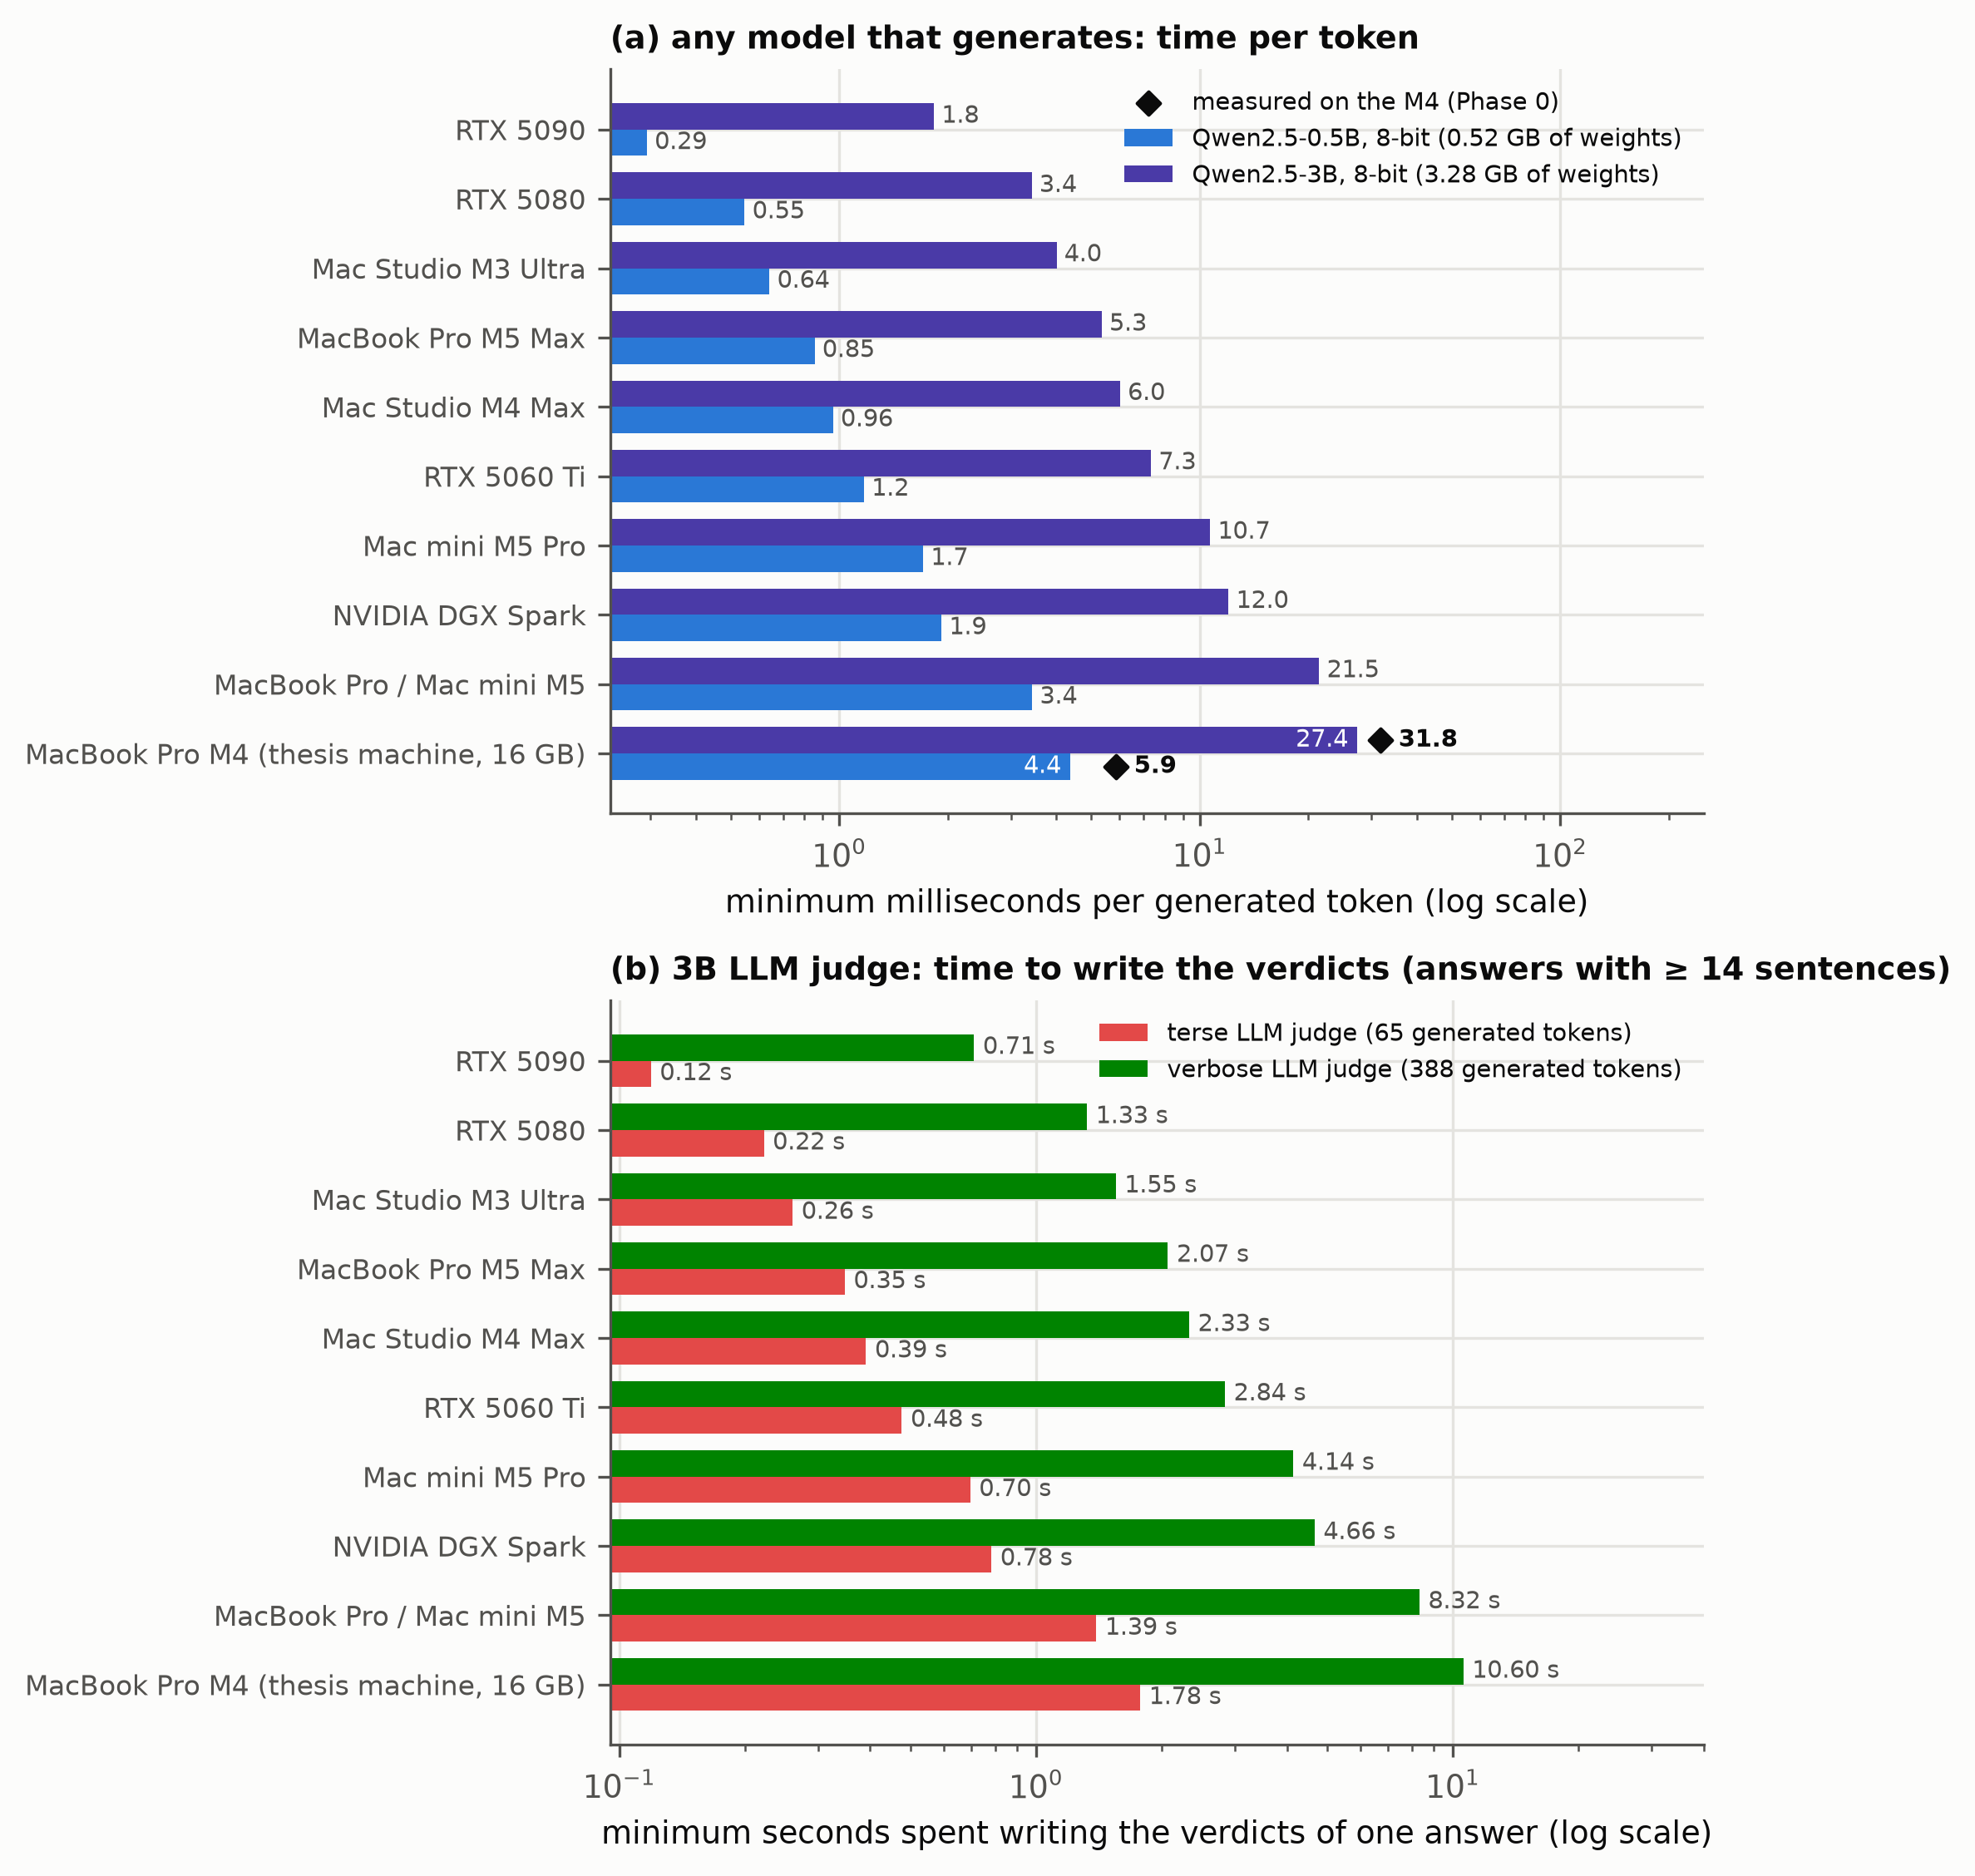
\includegraphics[width=\textwidth]{images/locality/decode_cost_by_hardware.png}
\caption{Lower bounds on the cost of generating text on each class of local hardware, computed as weight bytes divided
by the vendor's bandwidth (one request at a time; key-value cache ignored). (a) Time per generated token with the two
GroundOne base models in 8 bits; diamonds: decode time measured on the thesis machine. (b) Minimum time that a 3B
generative judge spends only on writing the verdicts for an answer of fourteen or more sentences (median generated tokens
of the latency protocol). A decision model generates no token, so both costs are zero for it on every machine.}
\label{fig:local-floor}
\end{figure}

\section{Runtimes and quantisation}
\label{sec:local-software}

\subsection{Runtimes}
\label{sec:local-runtimes}

The software for local inference has matured quickly. llama.cpp provides inference in C and C++ without external
dependencies, with quantisation and support for most consumer accelerators~\cite{llamacpp}. It also defined the GGUF
format, which gathers in a single file the quantised model and everything needed to use it, such as the tokenizer and
the conversation format. Tools such as Ollama and LM Studio build on it and reduce downloading and starting a model to a
single command. MLX is a computing framework designed by Apple for the unified memory of its processors, with an
interface close to NumPy~\cite{mlx2023}. Its language-model package supports quantisation and LoRA fine-tuning directly
on the device~\cite{mlxlm}, and it is the runtime used throughout this thesis.

The runtime matters as much as the chip. A comparison of five runtimes on the same Apple machine reports decoding rates
that differ by more than an order of magnitude, with MLX and MLC-LLM at the top and PyTorch's generic Metal back end at
the bottom~\cite{rajesh2025apple}; the study's numbers are not fully consistent with each other and should be read as
indicative, but the spread is large enough to survive the uncertainty. On phones, an evaluation of several runtimes and
devices finds large differences in speed, energy and thermal behaviour between runtimes and between
devices~\cite{laskaridis2024melting}.

\subsection{Specialised inference engines}
\label{sec:local-engines}

Next to the general runtimes, a second family of software appeared in 2026: inference engines written for a few models,
which give up generality to push further the memory limits described in Section~\ref{sec:bg-inference}. DwarfStar (ds4),
developed by Salvatore Sanfilippo, is a native engine optimised for a few large open-weight models, starting from DeepSeek
V4 Flash, and aimed at Macs with at least 96\,GB of memory, the DGX Spark and Strix Halo machines~\cite{antirez2026ds4}.
Two of its choices concern this thesis directly. The first is a key-value cache saved on disk: a conversation that has
already been read can be resumed without repeating the prefill, which for models of this size is the most expensive part
of a long request. The second is reading the weights directly from the SSD, which makes it possible to run models larger
than the available memory, at the price of speed.

Colibri takes this second idea to the extreme~\cite{justvugg2026colibri}. It exploits the fact that a mixture-of-experts
model uses only a small part of its weights for each token: it keeps the always-active part in memory and reads the experts
from disk when the router requests them. In this way GLM-5.2, a model of 744 billion parameters, runs on a laptop with
25\,GB of memory. The price is the one predicted by the cost model: the bandwidth of an SSD is a few gigabytes per second,
far below that of memory, and according to the authors generation drops to 0.05--0.1 tokens per second when cold on that
laptop and to 1.83 tokens per second on a 128\,GB Strix Halo machine~\cite{justvugg2026colibri}. It is the idea of LLM in a
flash~\cite{alizadeh2024flash} applied to expert models: memory capacity stops being a hard limit and turns into a
bandwidth limit, an even stricter one. Figure~\ref{fig:local-ssd}
illustrates the mechanism.

\begin{figure}[!htbp]
\centering
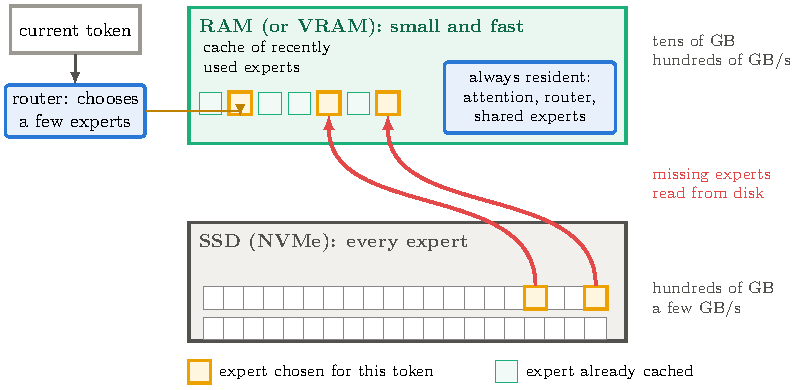
\includegraphics[width=\textwidth]{images/diagrams/ssd_streaming_tikz.pdf}
\caption{Streaming experts from the SSD in an engine such as Colibri. Memory holds the part of the model used by every
token (attention, router, shared experts) and a cache of recently used experts; every expert is stored on the SSD. For
each token the router chooses a few experts: those already cached are used at once, the missing ones are read from disk,
at a bandwidth of a few gigabytes per second. For example, GLM-5.2 keeps about 10\,GB resident and leaves about 429\,GB of
weights on disk~\cite{justvugg2026colibri}. The diagram is not to scale.}
\label{fig:local-ssd}
\end{figure}

Colibri matters to this thesis for a second reason. It exposes the same System One interface as Jev, through which any
model it runs answers closed questions by reading the probability of each option instead of generating the answer, and it
includes three decision models natively: Laya, GLiNER2.5-Decide and Clef~\cite{justvugg2026colibri}. The authors report
that, with Qwen3.6, four questions about the same document are answered 5.7 times faster than by generating the same
answers on the same CPU. This is a figure reported by the project and not verified in this thesis, obtained with a
different model and hardware, but it points in the same direction as the results of Chapter~\ref{sec:results}. That an
engine designed to run huge models on modest hardware adopts the reading of decisions as a first-class mode confirms that
the decision-model idea is spreading precisely where generation costs the most.

\subsection{Quantisation}
\label{sec:local-quantisation}

Quantisation stores the weights with fewer bits than the 16 used in training. On local hardware it serves two purposes
at once: the model fits in less memory, and decoding becomes faster, because decoding time is dominated by reading the
weights. Table~\ref{tab:local-quant} summarises the methods that shaped the field.

\begin{table}[htbp]
\centering
\caption{Weight quantisation methods for language models.}
\label{tab:local-quant}
\small
\begin{tabularx}{\textwidth}{@{}lXl@{}}
\toprule
Method & Idea and main result & Source \\
\midrule
LLM.int8() & 8-bit weights and activations; the few dimensions with very large anomalous values (outliers) are kept in
16 bits. No loss up to 175B parameters; saves memory but does not speed up small models. & \cite{dettmers2022llmint8} \\
GPTQ & 3--4-bit weights, quantised layer by layer by estimating how much each weight affects the error. 4-bit OPT-175B
loses 0.03 perplexity$^{a}$; small models lose more; 3.2--4.5$\times$ faster decoding from
bandwidth. & \cite{frantar2023gptq} \\
AWQ & 4-bit weights; the 1\,\% of channels that matter most, found from activation magnitudes, are protected by scaling.
Robust to the calibration data; designed for on-device use. & \cite{lin2024awq} \\
GGUF k-quants & 2--8-bit block formats of llama.cpp, the de facto standard for consumer distribution. & \cite{llamacpp} \\
MLX affine & 4- or 8-bit weights with a scale and a bias per group of 64; supports LoRA training on the quantised model
(used in this thesis). & \cite{mlxlm} \\
QLoRA & 4-bit normal-float base model with 16-bit adapters, for fine-tuning on limited memory. & \cite{dettmers2023qlora} \\
\bottomrule
\end{tabularx}

\smallskip
{\footnotesize\raggedright $^{a}$\,\emph{Perplexity} measures how well a model predicts a text: the lower it is, the less
the model is ``surprised'' by the words it encounters.\par}
\end{table}

Two results from this literature matter for this thesis. The first is that quantisation helps the bandwidth-bound phase.
GPTQ attributes its speed-ups entirely to the matrix-vector products of decoding and explicitly obtains no reduction in
computation~\cite{frantar2023gptq}; AWQ illustrates the same point with a roofline: on a desktop graphics card, a
200-token prefill takes 10 milliseconds while generating 20 tokens takes 310~\cite{lin2024awq}. Reducing the bits of the
weights therefore accelerates a model that generates far more than one that only reads. The second is that small models
are more fragile. GPTQ loses much more accuracy at 4 bits on a 1.3-billion-parameter model than on a 175-billion one, and
models of three billion parameters or fewer become unusable at 3 bits on phones~\cite{frantar2023gptq,laskaridis2024melting}.
LLM.int8() shows that a handful of outlier features control a large share of the attention probability
mass~\cite{dettmers2022llmint8}. For a model whose output is a probability that must be calibrated, rather than a text
that must merely be fluent, these observations argue for a conservative precision: GroundOne uses 8-bit weights. A measurement made in this thesis
confirms that, at this precision, quantisation costs no accuracy: applying the same adapter of the 0.5B model to the
original 16-bit weights leaves the three-way balanced accuracy on T1 practically unchanged (0.768 against 0.769), the
probabilities change by 0.011 on average and the predicted class agrees on 98\,\% of the sentences
(Section~\ref{sec:results-locality}).

\subsection{Faster generation without fewer tokens}
\label{sec:local-speculative}

A different family of methods accelerates generation without changing the model. In speculative decoding, a small draft
model proposes several tokens, and the large model checks all of them in a single forward pass, accepting the longest
prefix that it would have produced itself; the output is identical to that of the large model, and the speed-up reaches
two to three times~\cite{leviathan2023speculative}. The method is useful for any system that must generate, but it
does not change the nature of the cost: every accepted token still requires a forward pass of the large model, and the
total amount of computation grows~\cite{leviathan2023speculative}. It makes writing cheaper; it does not make it free.

\section{Energy}
\label{sec:local-energy}

On a battery-powered device, energy is a property of the method, not only of the hardware. Measurements on datacenter
hardware show that the energy of a request grows with the number of generated tokens and depends strongly on model size
and task~\cite{samsi2023words,luccioni2024power}. On phones, a 3-billion-parameter model in 4 bits spends between 0.58 and
0.76 joules per generated token, with sustained power around 14\,W and surface temperatures close to
48\,\textdegree C~\cite{laskaridis2024melting}; a rule of thumb from work on small models puts the cost at about 0.1 joules
per generated token for each billion parameters~\cite{liu2024mobilellm}. Moving the prefill to a phone's NPU
reduces its energy by 1.9 to 4.3 times with respect to the graphics unit~\cite{xu2025npu}.

The distinction between the two phases also applies to power. Prefill keeps the arithmetic units busy and draws more
power; decoding waits for memory and draws less, but for much longer~\cite{patel2024splitwise}. A method that
saves time therefore saves energy too, but by a smaller factor, and Chapter~\ref{sec:results} measures exactly this
effect: GroundOne spends 5.5 joules per long answer with the 0.5B model and 33 with the 3B, less than any generative
judge of the same size, but with an advantage smaller than in time (Section~\ref{sec:results-energy}).

\section{Consequences for verification on the device}
\label{sec:local-verification}

The chapter can now be summarised in one observation: on a local device, which serves one request at a time, reading a
token costs far less than writing one, fourteen to sixteen times less on the thesis machine
(Sections~\ref{sec:local-phases}--\ref{sec:local-floor}), and recent hardware generations accelerate reading much more
than writing (Section~\ref{sec:local-asymmetry}). This has a direct consequence for a verifier that runs next to the generator.

A generative judge verifies an answer by reading the document and the answer and then writing its verdicts. It pays a
prefill, like any method that reads the document, and then one decoding step for every token it writes. In the latency
protocol of this thesis (Section~\ref{sec:results-latency}), a terse 3B judge writes a median of 65 tokens for an answer of
fourteen or more sentences, and a verbose one, which explains each verdict, writes 388. The lower bound of
Section~\ref{sec:local-floor} turns these counts into a minimum time that no implementation can beat
(Figure~\ref{fig:local-floor}b): on the thesis machine, at least 1.8 seconds for the terse judge and 10.6 for the verbose
one, on top of the prefill; even on the fastest graphics card, 0.12 and 0.71 seconds.

A decision model removes this term altogether. It reads the document and the answer once and takes every decision from the
logits computed during that single reading, so its cost is the prefill alone: the compute-bound phase, the one that
local hardware performs well and that new hardware accelerates most. Its advantage over a judge is therefore not a
property of one machine but of the cost structure of local inference, and it is largest exactly where inference is local.
Locality, which at first sight is only a constraint on the size of the model, becomes the reason why the design matters.

Three requirements for the verifier follow from this chapter, and they guide the method of Chapter~\ref{sec:method}. It
must generate no tokens, so that its cost is a single prefill. It must use a model small enough to share a 16\,GB machine
with a generator and a retriever, quantised conservatively because its output is a probability. And it must read its
decisions from logits, which only a local model exposes, so that they can be calibrated.
